% \clearpage
\section{Results \& Discussion}

	For all the simulation, the main convergence criterion is that the variance of the ground state $\delta \ket\psi$, computed by
	\be \delta \ket\psi = \ev{\mc H^2}{\psi} - \ev{\mc H}{\psi}^2 \ee
	must be below the threshold $\delta \ket \psi < 10^{-8}$ hence, except explicit mention, $\delta \ket \psi \sim 10^{-9}$ is taken.

	Once the main part of the DMRG simulation was coded, it was tested on the TFI model to retrieve the first results that were concerning the central charge. The central charge of a Virasoro minimal model labelled by the two integers $(p,q)$ is given by \cite{francesco1997}
	\be c = 1 - 6\frac{(p-q)^2}{pq} \ee
	The first non-trivial unitary model is given by $(4, 3)$ and is the critical TFI \cite{francesco1997}, whose central charge is then $c = \frac 1 2$. The next one that will be sought for is the TCI labelled by $(5, 4)$ \cite{francesco1997, friedan1985, friedan1984}, whose central charge is then $c = \frac{7}{10}$.

	Having that said, the results obtained regarding the central charge for critical TFI with $[ff]$ OBCs are presented on \autoref{fig:cTFI}. As it can be observed on \autoref{fig:cTFI.a}, the corresponding formula for entanglement entropy \eqref{eq:cardyOBCs} greatly fits the data obtained for chain of length $L=100$, and allows to recover the central charge $c = 0.50715 \pm 0.00003$, which is a very good estimate for the expected central charge for critical TFI standing in the Ising CFT universality class. Repeating this procedure for several lengths yields the extrapolation of $c$ in $\frac 1 L$ in \autoref{fig:cTFI.b} which seemingly is a good regression with $R^2 = 0.99998$. Hence, for $L \to \infty$, the intercept tells $c=0.50016 \pm 0.00003$, giving a better estimate for $c$ of critical TFI and confirms it is described by Ising CFT.

	\begin{figure}[h!]
		\hspace{-0.4cm}
		\subfloat[]{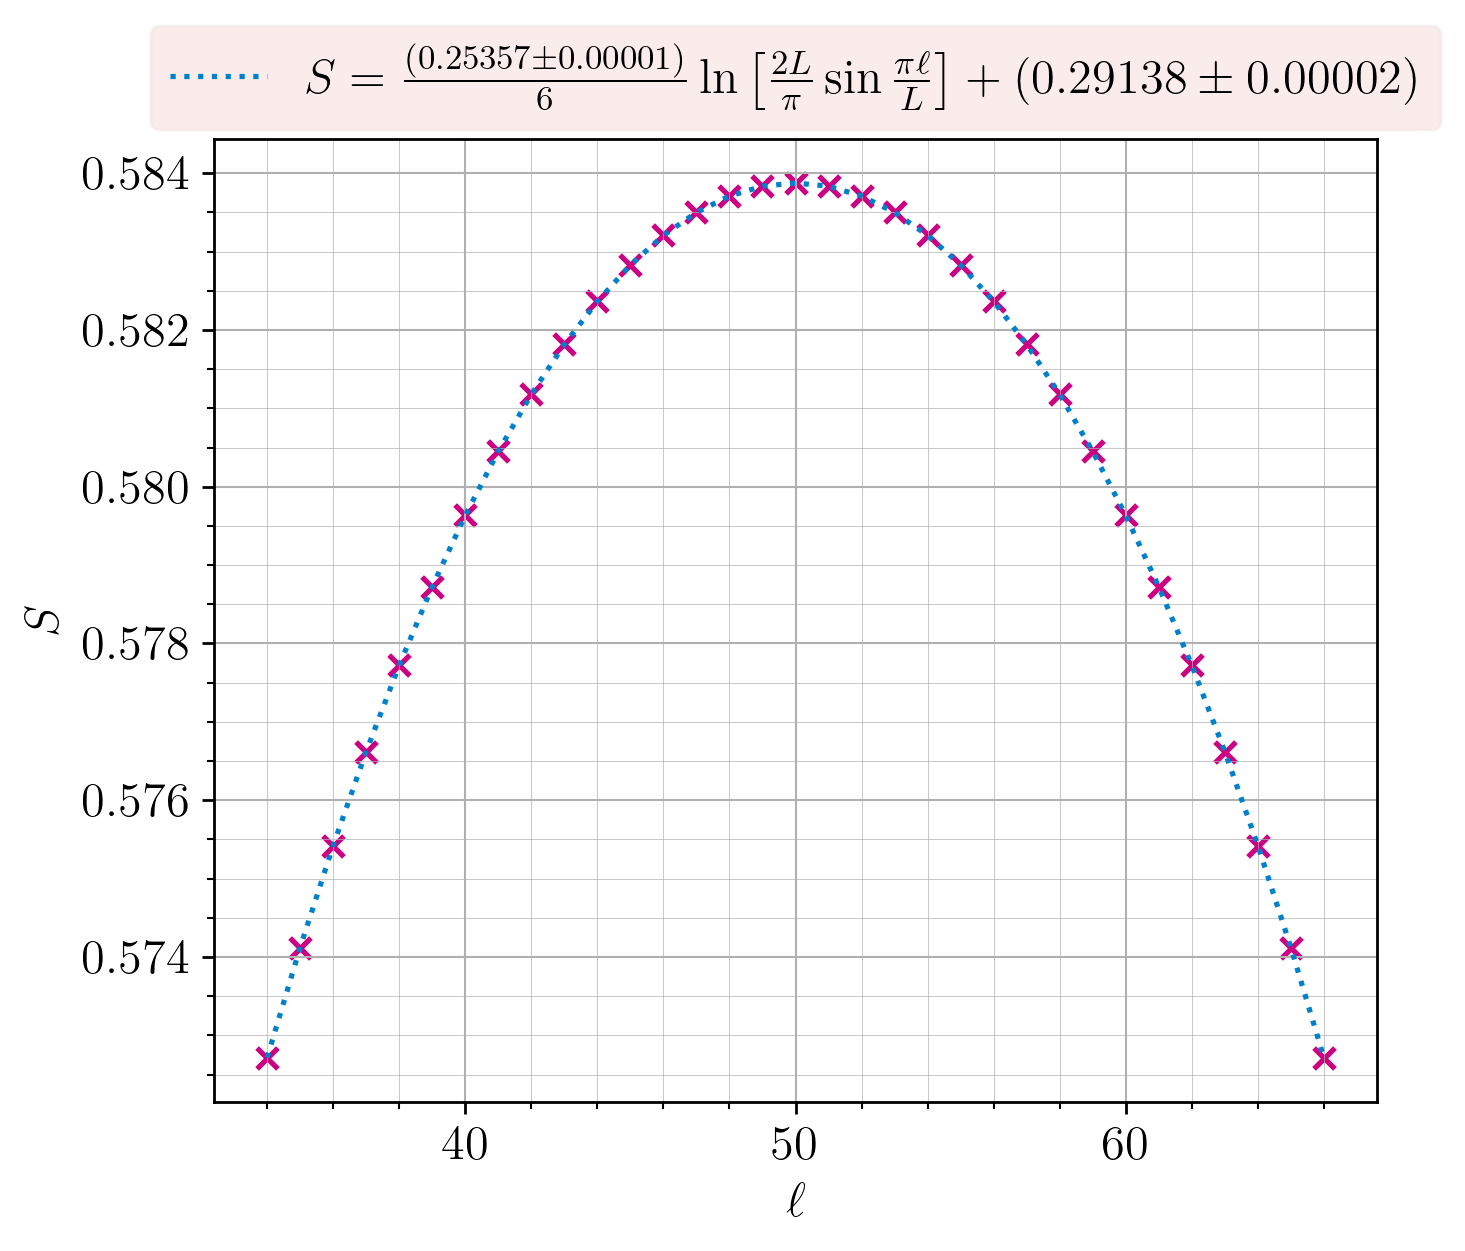
\includegraphics[scale=0.66]{../graphs/entropies/ff/alone_L=100.0_chi=100.0_J=1.0_h=1.0_i=1.0_3=0.0_c=0.0.png}\label{fig:cTFI.a}}\
		\subfloat[]{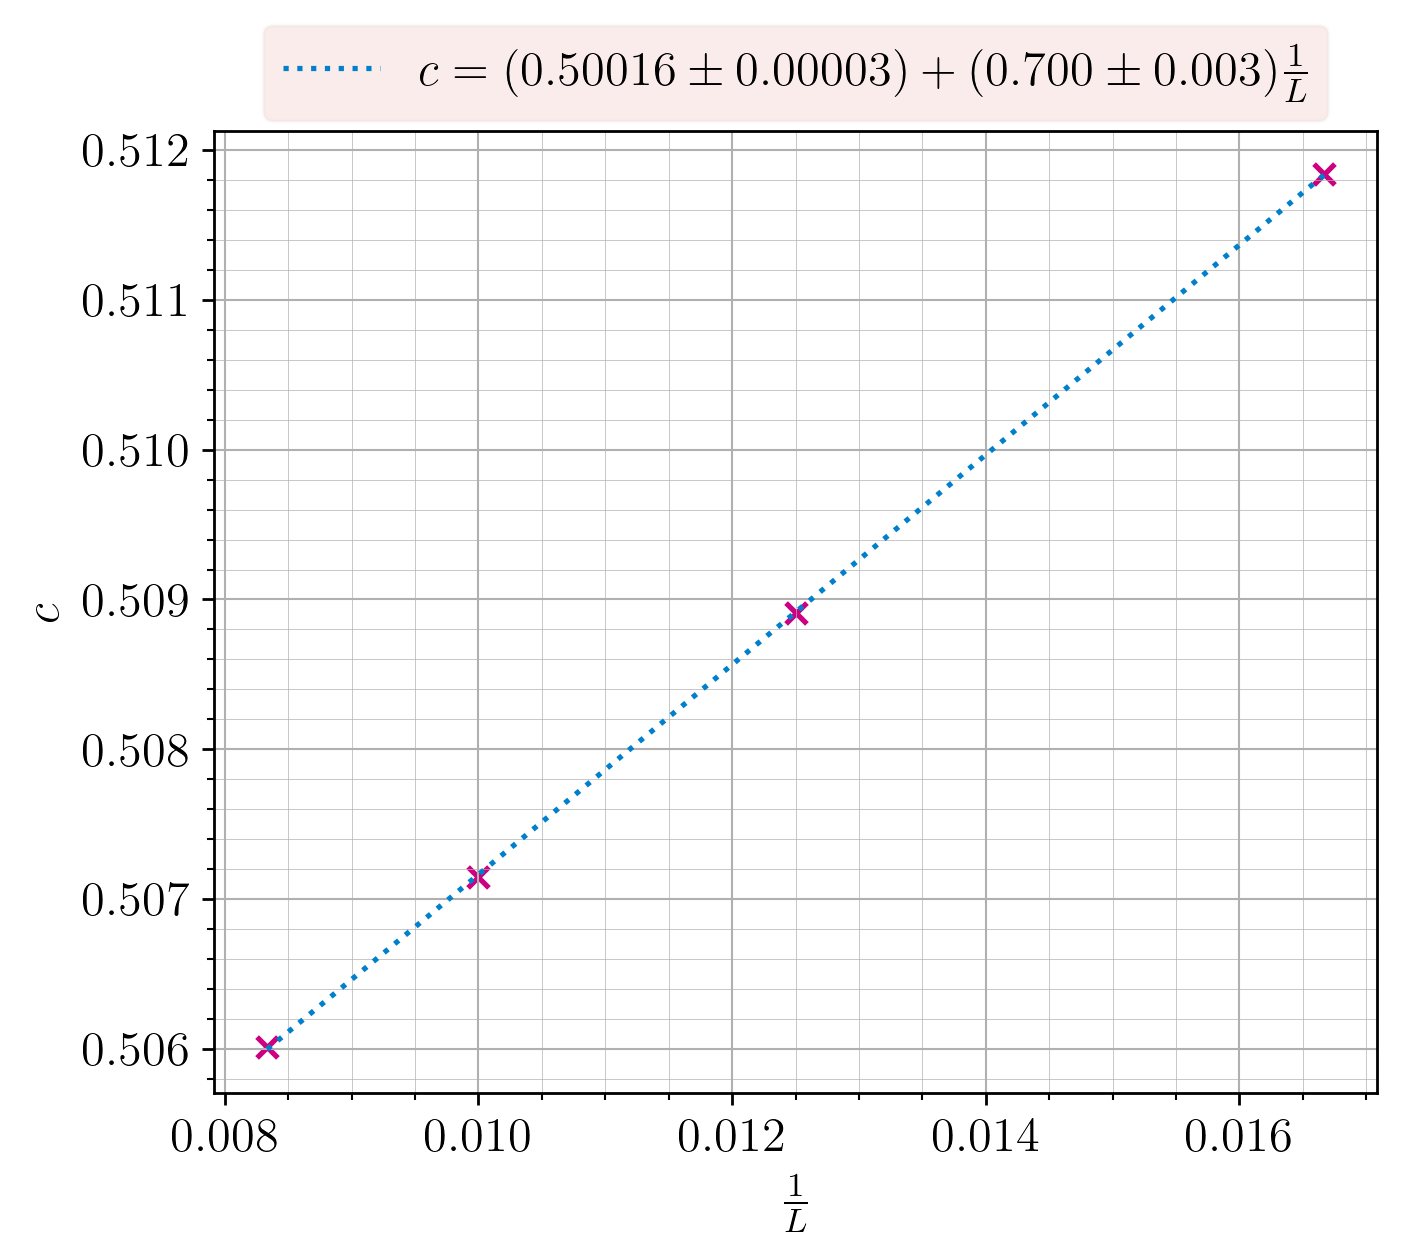
\includegraphics[scale=0.66]{../graphs/entropies/ff/calabrese_chi=100.0_J=1.0_h=1.0_i=1.0_3=0.0_c=0.0.png}\label{fig:cTFI.b}}
		\caption{Critical TFI with $\chi=100$ and $[ff]$ OBCs. (a): Typical fitting of the entanglement entropy with Cardy-Calabrese formula \eqref{eq:cardyOBCs} for $L=100$. (b): Extrapolation of the central charge.}
		\label{fig:cTFI}
	\end{figure}

	Noticing the expected value of central charge is obtained for critical TFI, it can be expected to obtain the correct central charge too for the OF model \eqref{eq:OF} for $\lambda_3/\lambda_I = 0.856$. According to \cite{obrien2018}, this point is described by TCI CFT, which has $c=7/10$. Therefore, \autoref{fig:cTCI} shows the results of the extrapolation of $c$ in $1/L$ for $[ff]$ OBCs. Both extrapolations with different formulas to recover $c$ for different lengths do not lead to the expected value, but slightly above $c\sim 0.77$. There can be several explanations for this to happen. At first, even if not shown, the bond dimension $\chi$ has no role at this point since the exact same extrapolated value of $c$ has been obtained for $\chi=200$, therefore this assumption that for the range of values for the bond dimension acceptable for normal computer does not play any role in results shown on \autoref{fig:cTCI}.

	\begin{figure}[h!]
		\hspace{-0.4cm}
		\subfloat[]{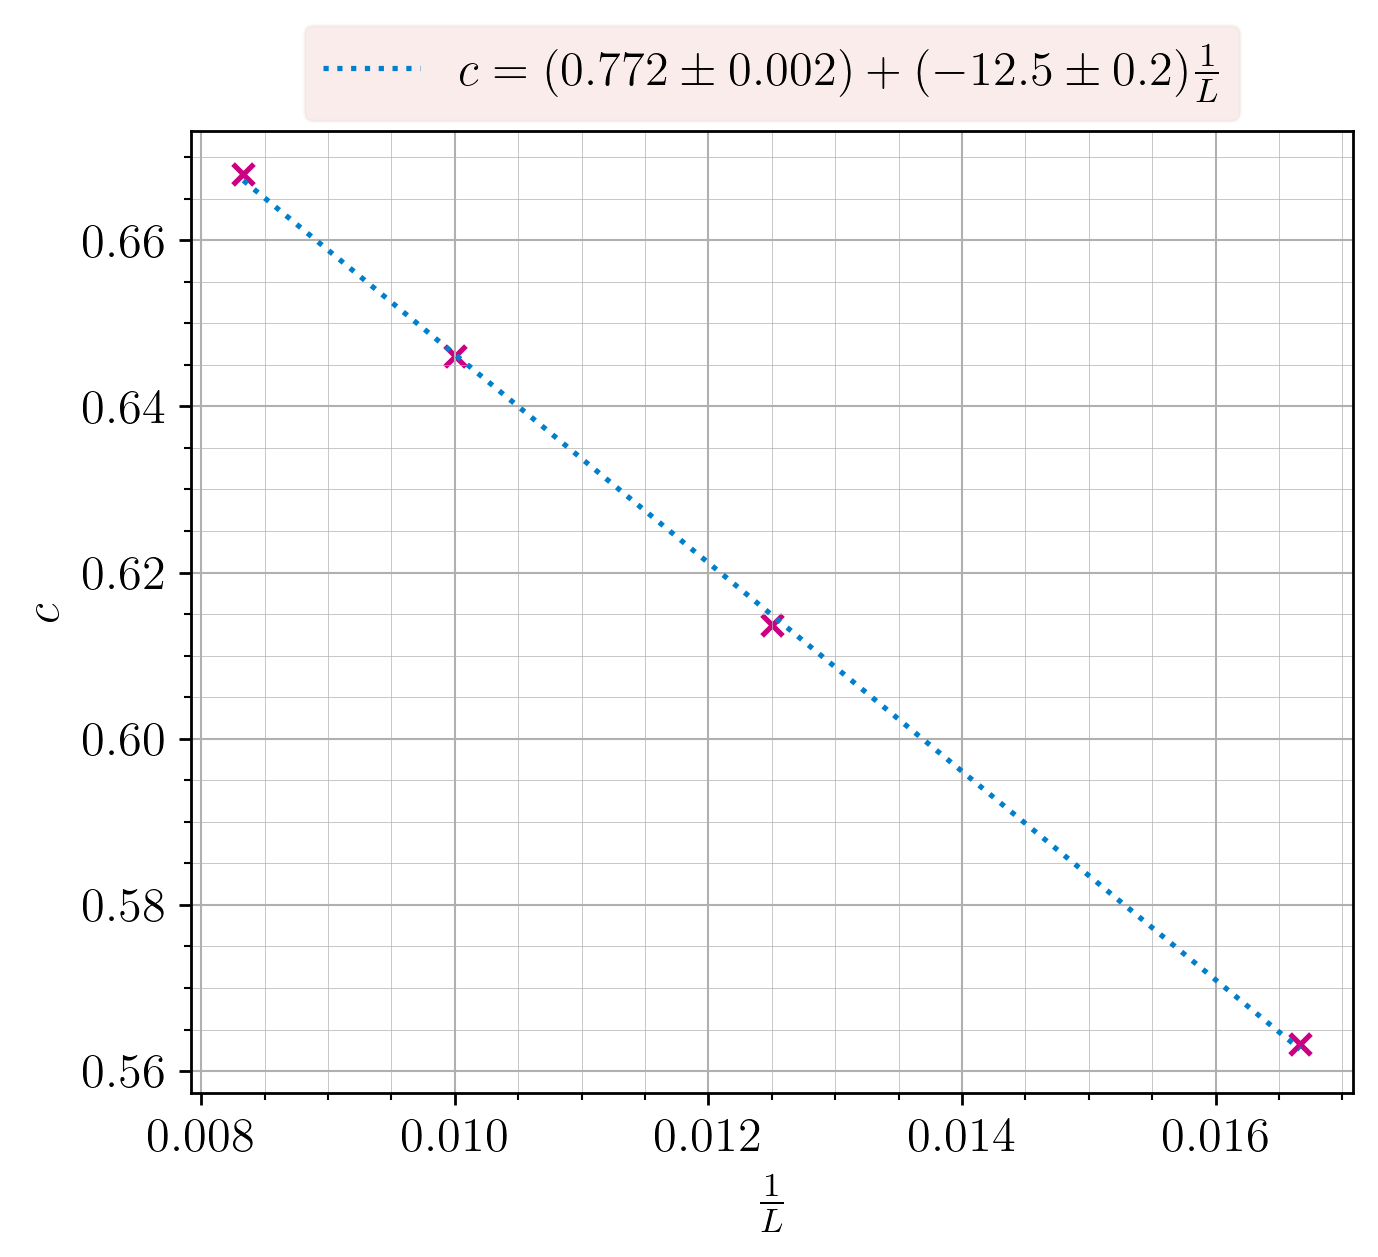
\includegraphics[scale=0.66]{../graphs/entropies/ff/calabrese_chi=100.0_J=1.0_h=1.0_i=1.0_3=0.856_c=0.0.png}\label{fig:cTCI.a}}\quad
		\subfloat[]{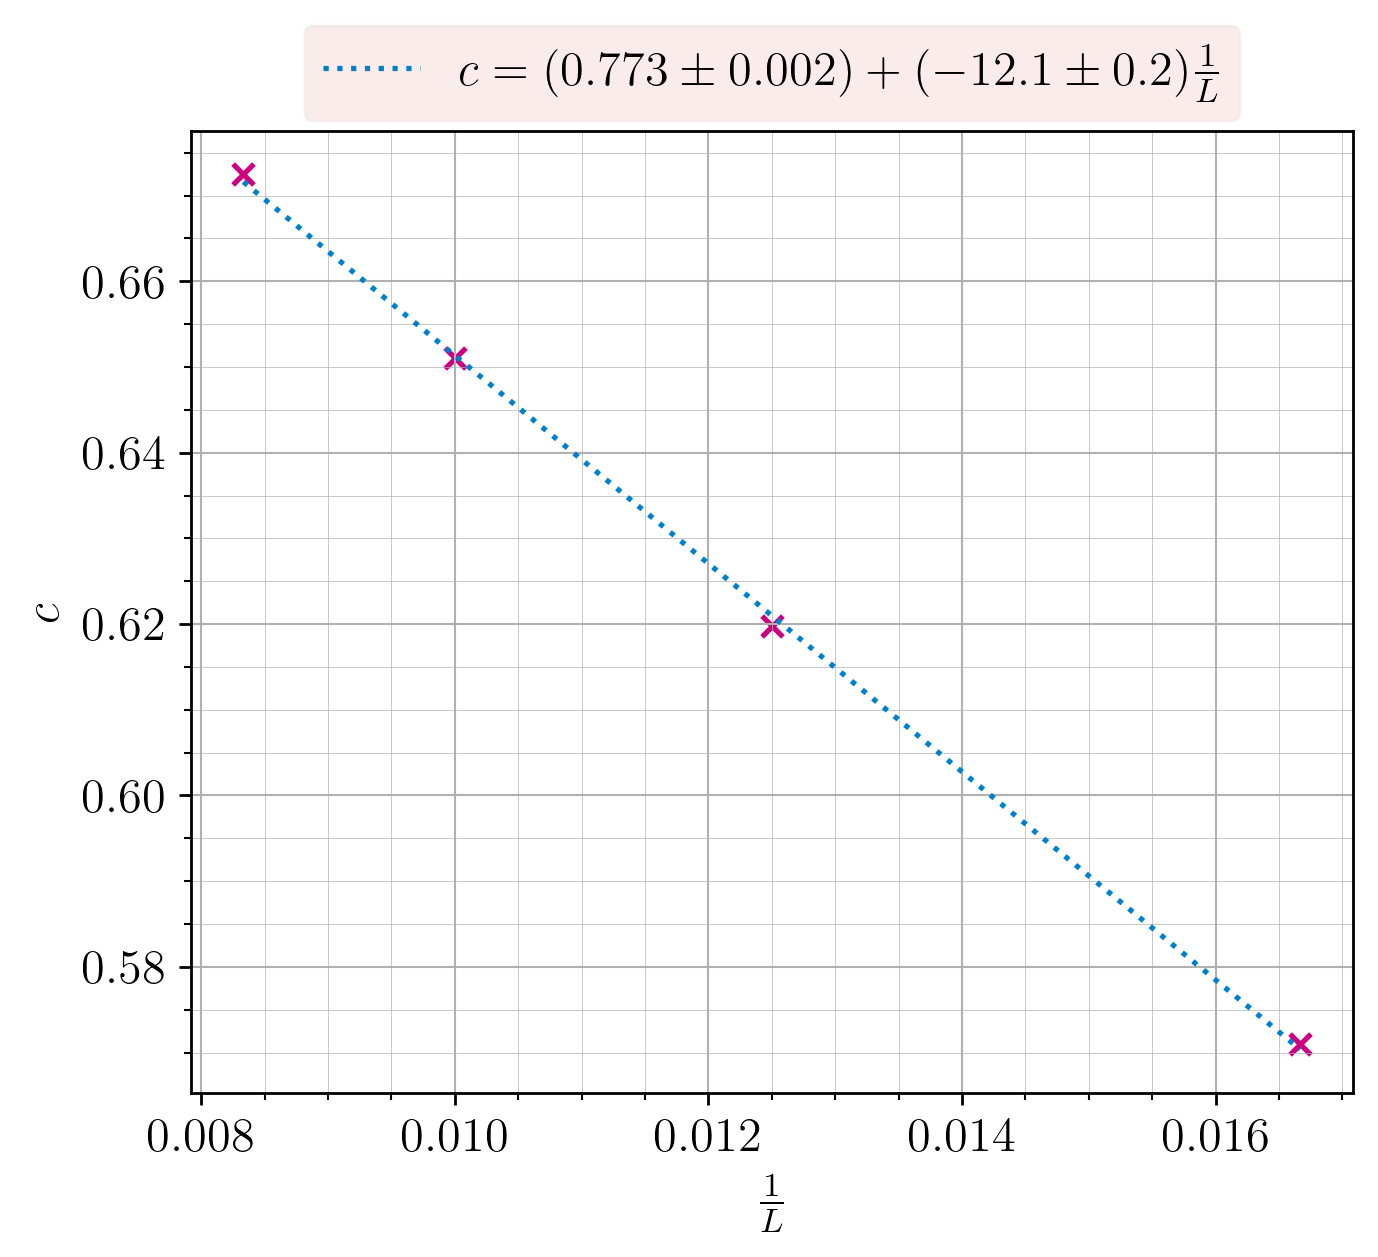
\includegraphics[scale=0.66]{../graphs/entropies/ff/other_chi=100.0_J=1.0_h=1.0_i=1.0_3=0.856_c=0.0.png}}
		\caption{Extrapolation of the central charge for $\lambda_3/\lambda_I=0.856$, $\chi=100$ and $[ff]$ OBCs (a): with Cardy-Calabrese formula \eqref{eq:cardyOBCs}. (b): with \eqref{eq:otherOBCs}.}
		\label{fig:cTCI}
	\end{figure}

	Hence, it can be useful to look at how the extrapolations of $c$ behave for different values of $\lambda_3/\lambda_I$, as in \autoref{fig:phaseOBCs}, for $[ff]$ OBCs. It is expected that $c =1/2$ for values $\lambda_3/\lambda_I \in [0, 0.856[$, $c=7/10$ for $\lambda_3/\lambda_I =0.856$ and $c=0$ for $\lambda_3/\lambda_I>0.856$ \cite{obrien2018}. The observation of the figure then tells a few things. For $0\leq \lambda_3/\lambda_I \leq 0.6$ the central charge follows a straight line in $1/L$ converging to $c\sim 0.5$ even though the linearity seems broken for small lengths for $\lambda_3/\lambda_I=0.6$. However, even if for $0.7\leq \lambda_3/\lambda_I \leq 0.82$ the convergence to $c\sim 0.5$ appears to still be present, the central charge passes through a maximum at a finite length, that has been checked to correspond to the moment the correlation length computed at the middle of the chain becomes equal to the length $L$ of the chain. % maybe expalain correlation length
	This behavior seems to be found again for $0.83\leq \lambda_3/\lambda_I \leq 0.85$ except that the length for which $c$ was computed are not large enough to observe a maximum but it can be inferred that it would appear for larger lengths. However, there is nothing compelling to say they must converge to $c\sim 0.5$. For $\lambda_3/\lambda_I=0.856$, the behavior found in \autoref{fig:cTCI.a} is repeated and the convergence to $c\sim 0.77$ also is. Finally, for $\lambda_3/\lambda_I=0.86$, a maximum is again reached but this time it can be expected that $c$ goes to $0$ for larger lengths, even though no conclusions can made. Overall, the \autoref{fig:phaseOBCs} shows that the behavior of $c$ in $1/L$ is incorrect, partially unexpected and no clear conclusion can be drawn. This can explain the incorrect value of the central charge in the TCI point found in \cite{obrien2018}.

	\begin{figure}[h!]
		\centering
		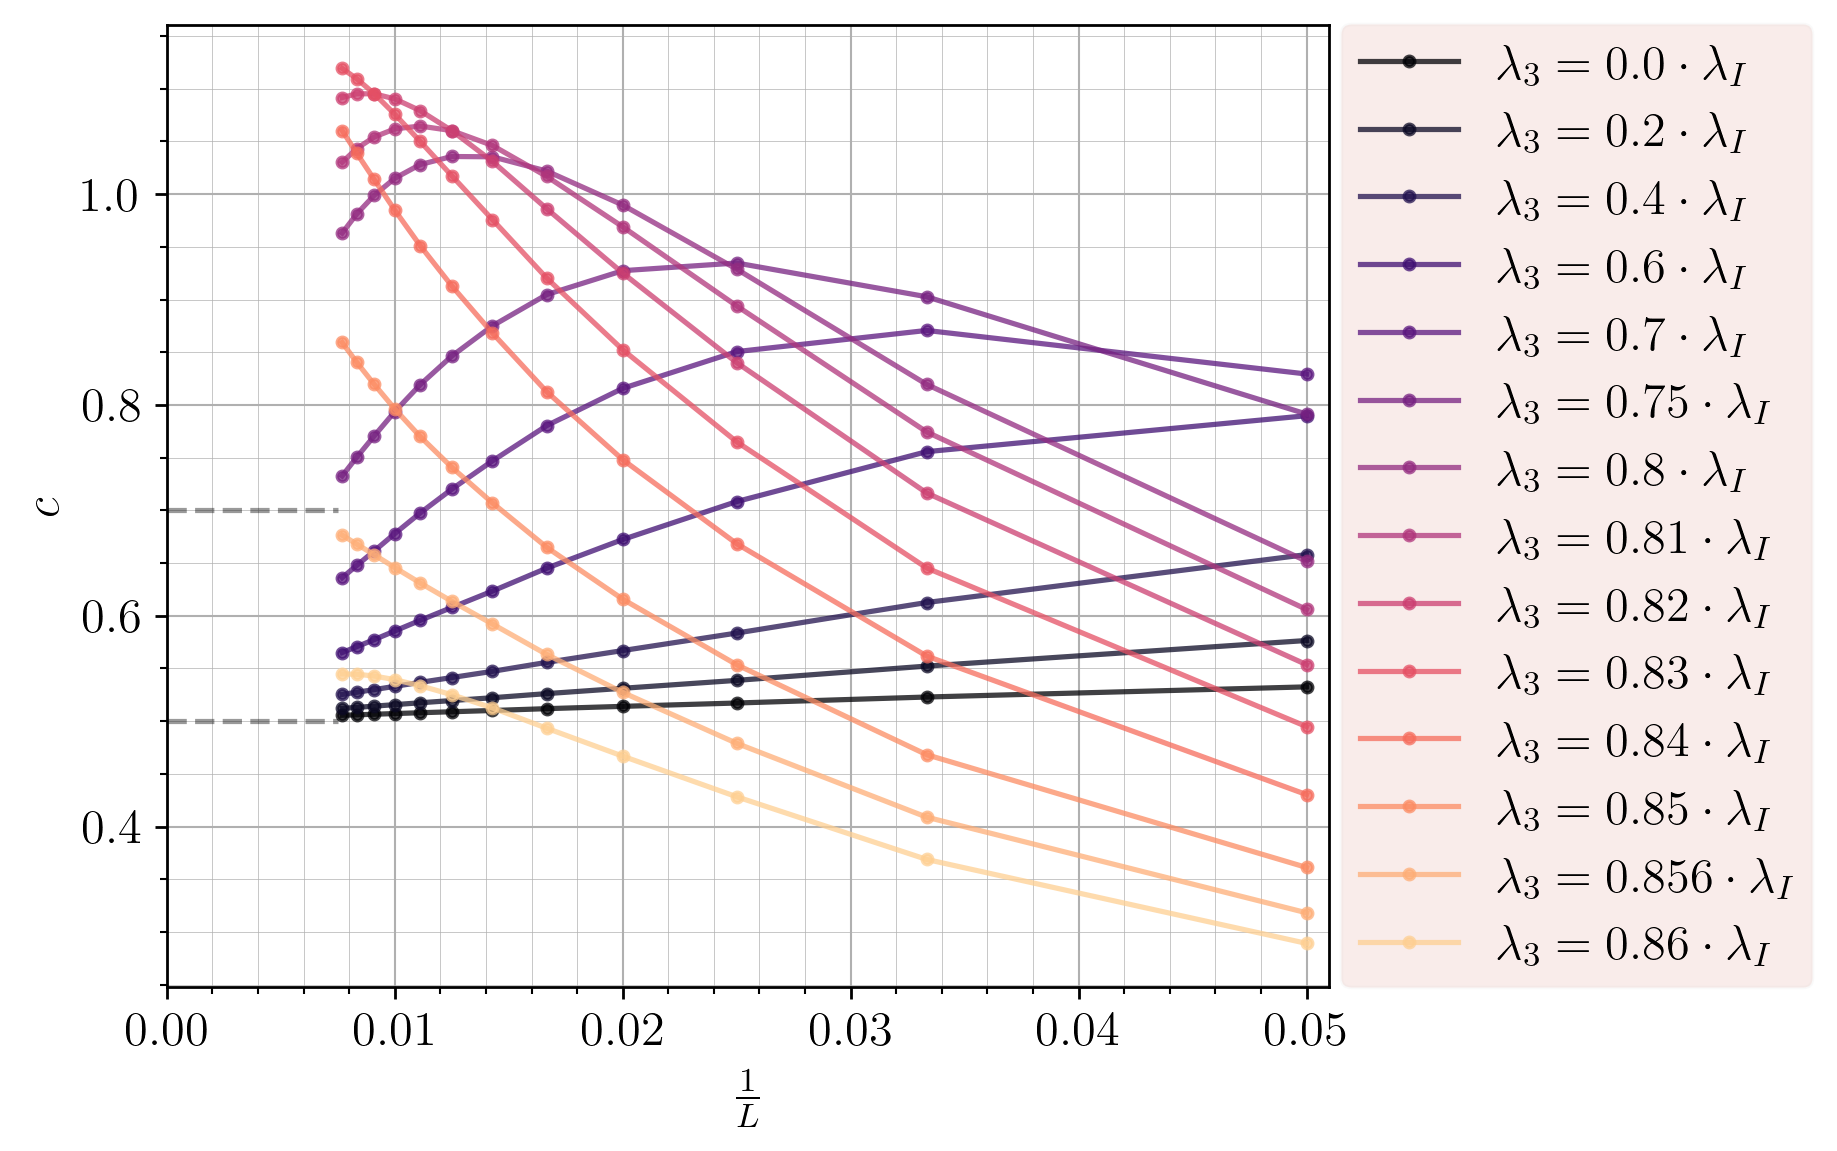
\includegraphics[scale=0.66]{../graphs/phase/ff/chi=100.0_J=1.0_h=1.0_i=1.0_c=0.0.png}
		\caption{Extrapolation of the central charge with Cardy-Calabrese formula \eqref{eq:cardyOBCs} as $\lambda_3/\lambda_I$ is varied with $\chi=100$ and $[ff]$ OBCs. Dashed grey lines are added as guides for $c=1/2$ and $7/10$.}
		\label{fig:phaseOBCs}
	\end{figure}

	The central charge reaching a maximum can be due to extra entanglement throughout the chain, coming from the edge states. % cite if possible
	To try to remove them, to pin the edge spins with on-site magnetic field can be efficient. 

	To find an adequate value of the pinning field for different boundary conditions presented on \autoref{tab:pinningBCs}, the spin expectation values at both boundary sites can be computed by changing the pinning field magnitude $h_\text{pin}$ in the $x$-direction. This is shown on \autoref{fig:edgesSpin} for $\lambda_3/\lambda_I=0.856$ and $L=30$. It can be noticed that the spins are totally aligned to the magnetic field for $|h_\text{pin}|>20$. To be certain of this, the value of $|h_\text{pin}|=100$ will be taken from now on. It can also be observed that the $[ff]$ OBCs let the edges spin alone with $\ev{\sigma^x_l}=0$, however for $[f-]$ OBCs the free edge acquires a small $\ev{\sigma^x_l}\sim -0.1$. It will be seen later on that this seems to not be problematic. It is worth mentioning moreover that \autoref{fig:edgesSpin} has been checked to neither be specific to the model used nor the length of the chain.

	\begin{figure}[h!]
		\centering
		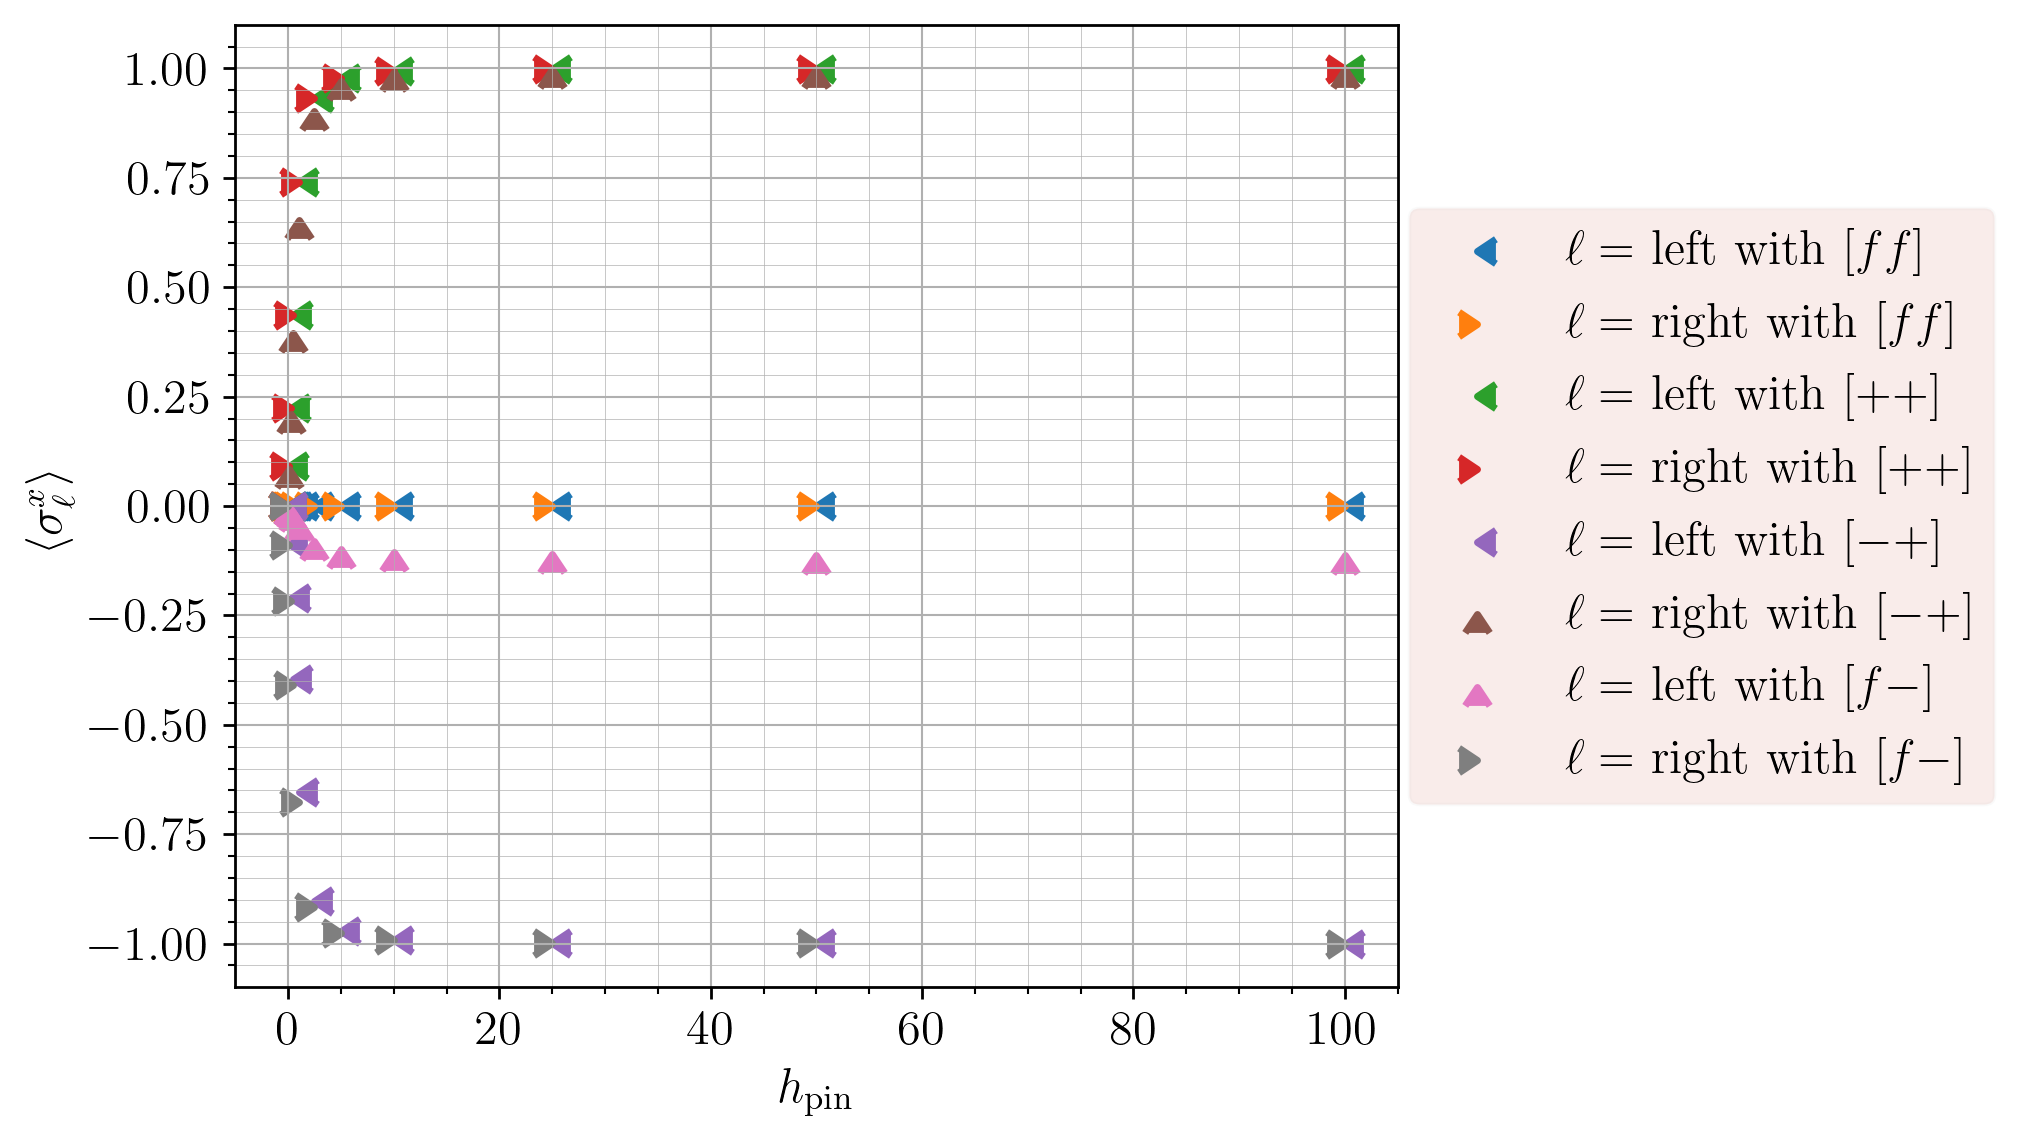
\includegraphics[scale=0.66]{../graphs/edge/L=30.0_chi=50.0_J=1.0_h=1.0_i=1.0_3=0.856_c=0.0.png}
		\caption{Spin at the edges of the chain while pinning them with various $h_\text{pin}$ magnitudes and under different OBCs for $L=30$, $\chi=50$ and $\lambda_3/\lambda_I=0.856$.}
		\label{fig:edgesSpin}
	\end{figure}

	To confirm that the pinning field does not break the behavior of the spins in the bulk, the spin expectation value in the middle of the chain is computed for multiple values of $h$ for TFI \eqref{eq:TFI} and different OBCs for $L=30$. The behavior is the exact one expected \cite{yang1951, pfeuty1970} through the transition at $J=h$ as seen in \autoref{fig:spinTFI}, with the $\langle \sigma^x_{L/2}\rangle$ having the correct sign in the ordered phase $h<J$ forced by the pinning field at the edges. Moreover, the behavior of the $\langle \sigma^x_{L/2}\rangle$ is fully expected \cite{pfeuty1970}. Therefore, the pinning of the edge spins seems to imply a correct behavior of the system at least for the TFI model.

	\begin{figure}[h!]
		\hspace{-0.4cm}
		\subfloat[]{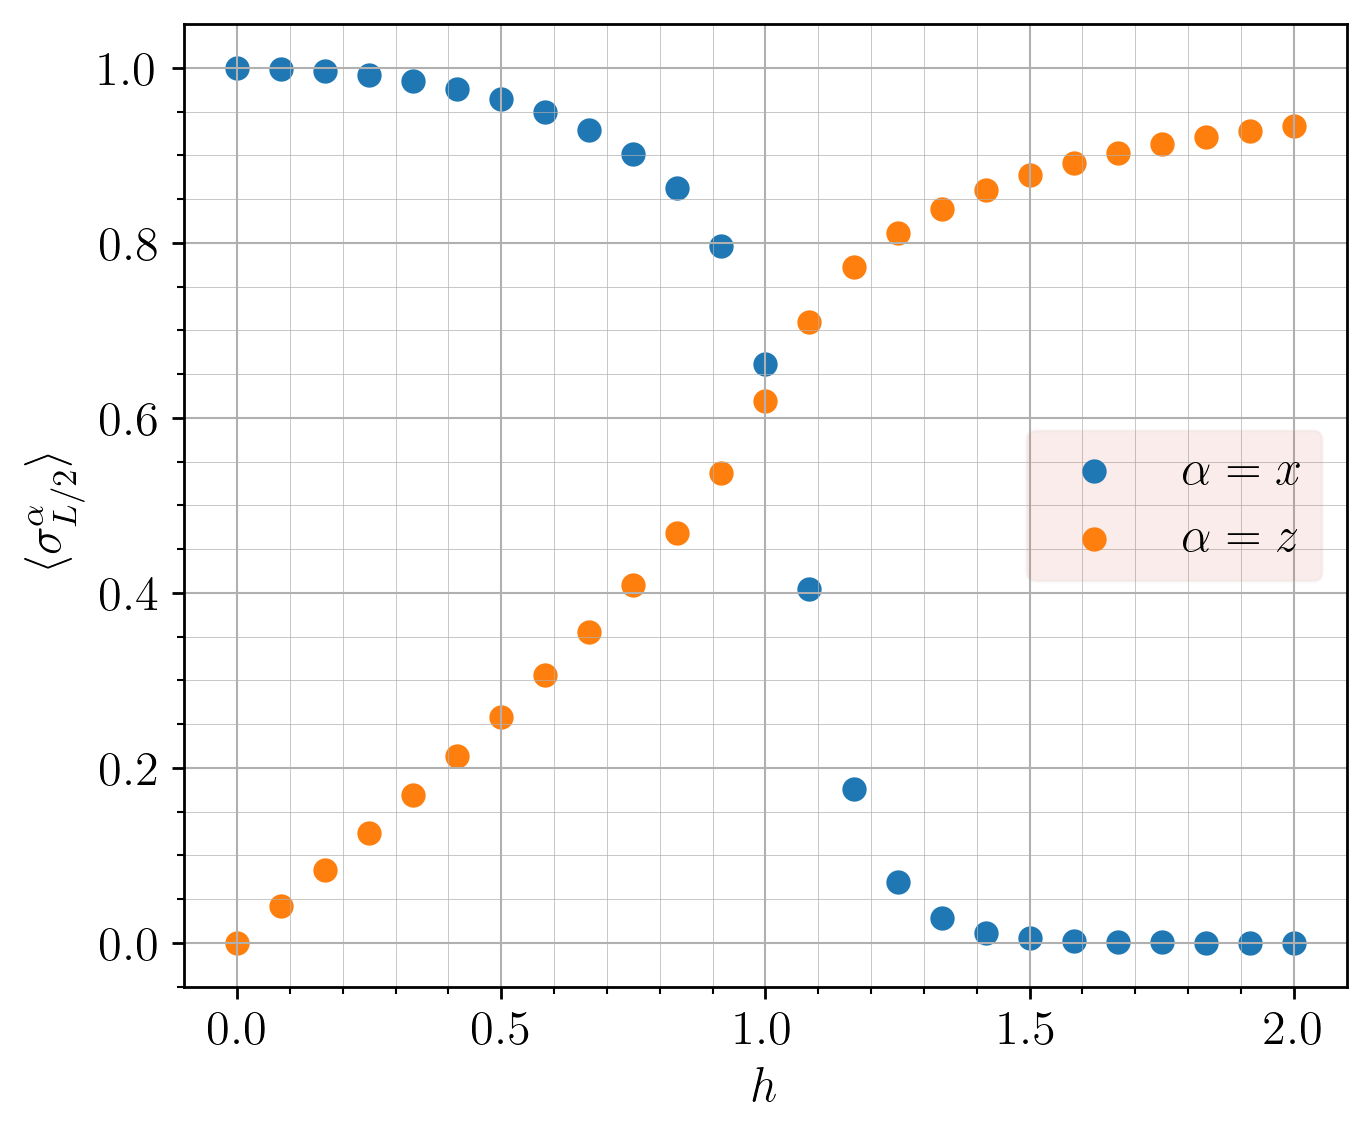
\includegraphics[scale=0.66]{../graphs/spin/--/100/L=30_chi=30.0_J=1.0_i=1.0_3=0.0_c=0.0.png}}\quad
		\subfloat[]{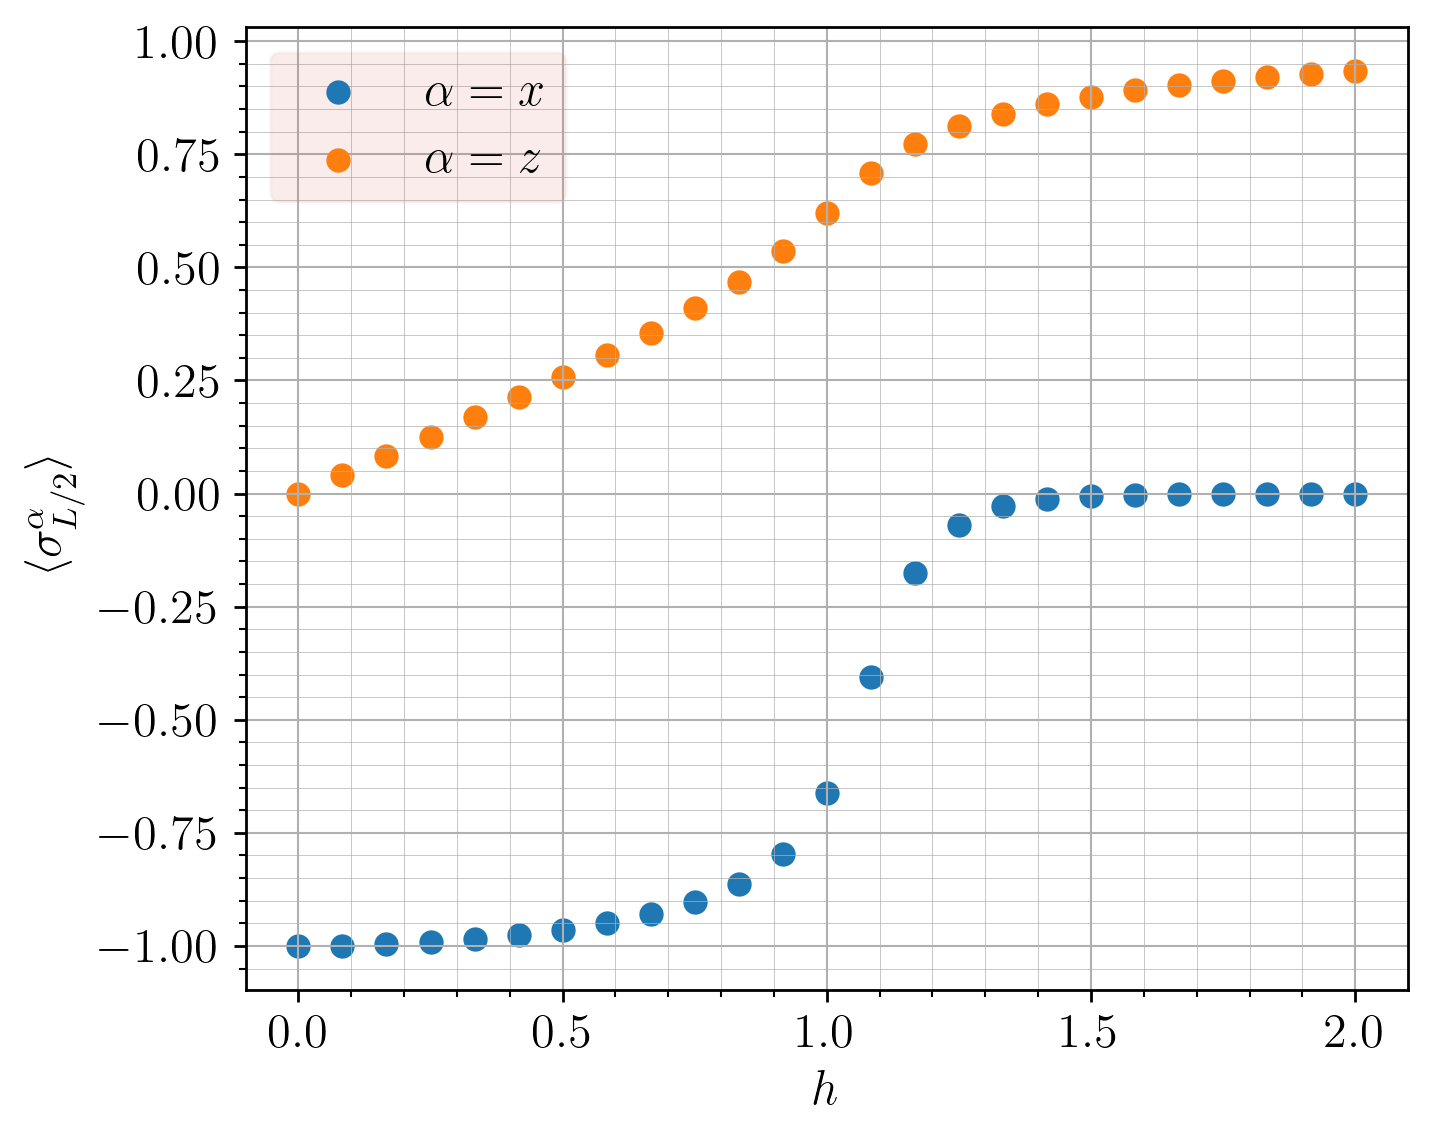
\includegraphics[scale=0.66]{../graphs/spin/++/100/L=30_chi=30.0_J=1.0_i=1.0_3=0.0_c=0.0.png}}
		\caption{Spin expectation values of TFI with $J=1$ in the middle of the chain for $L=30$ and $\chi=30$ (a): with $[++]$ OBCs and $h_\text{pin}=-100$. (b): with $[--]$ OBCs and $h_\text{pin}=100$.}
		\label{fig:spinTFI}
	\end{figure}

	To confirm further and try to find the correct value $c=7/10$ of the TCI CFT point $\lambda_3/\lambda_I=0.856$, the central charge is extrapolated for $[++]$ OBCs with $h_\text{pin}=100$. For critical TFI, the central charge is correctly recovered as $c=0.50029\pm 0.00008$ in the large $L$ limit. It can be noted that the slope in now negative as compared to the one on \autoref{fig:cTFI.b} where it is positive. This can from the reduce in entanglement entropy from pinning the edge spins. On the other hand, the result obtained for $\lambda_3/\lambda_I=0.856$ is $c= 0.594\pm 0.002$ which is even worse than the one obtained with $[ff]$ OBCs in \autoref{fig:cTCI.a} being $c=0.772 \pm 0.002$. The linearity seems to be slightly off this time even if still acceptable with $R^2=0.999$, but it exhibits the fact that this pinning has strongly affect the system and the linear regression might no be correct, at least for such small lengths.

	\begin{figure}[h!]
		\hspace{-0.4cm}
		\subfloat[]{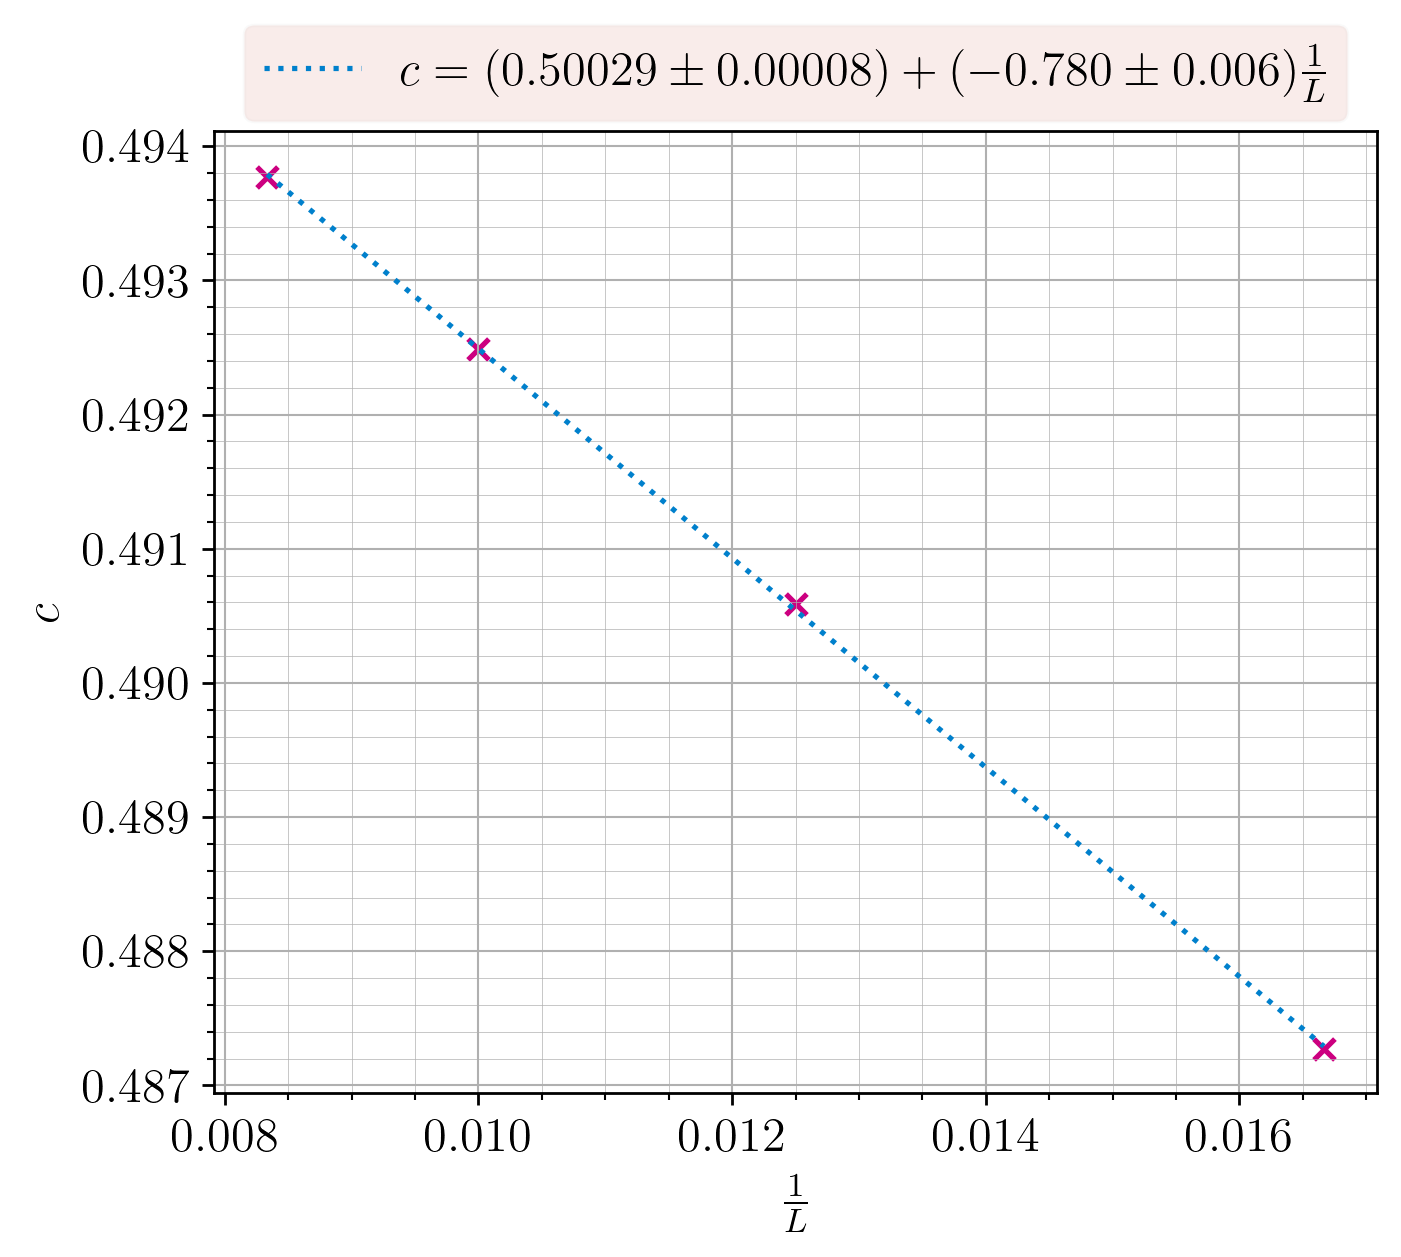
\includegraphics[scale=0.66]{../graphs/entropies/--/100/calabrese_chi=100.0_J=1.0_h=1.0_i=1.0_3=0.0_c=0.0.png}}\quad
		\subfloat[]{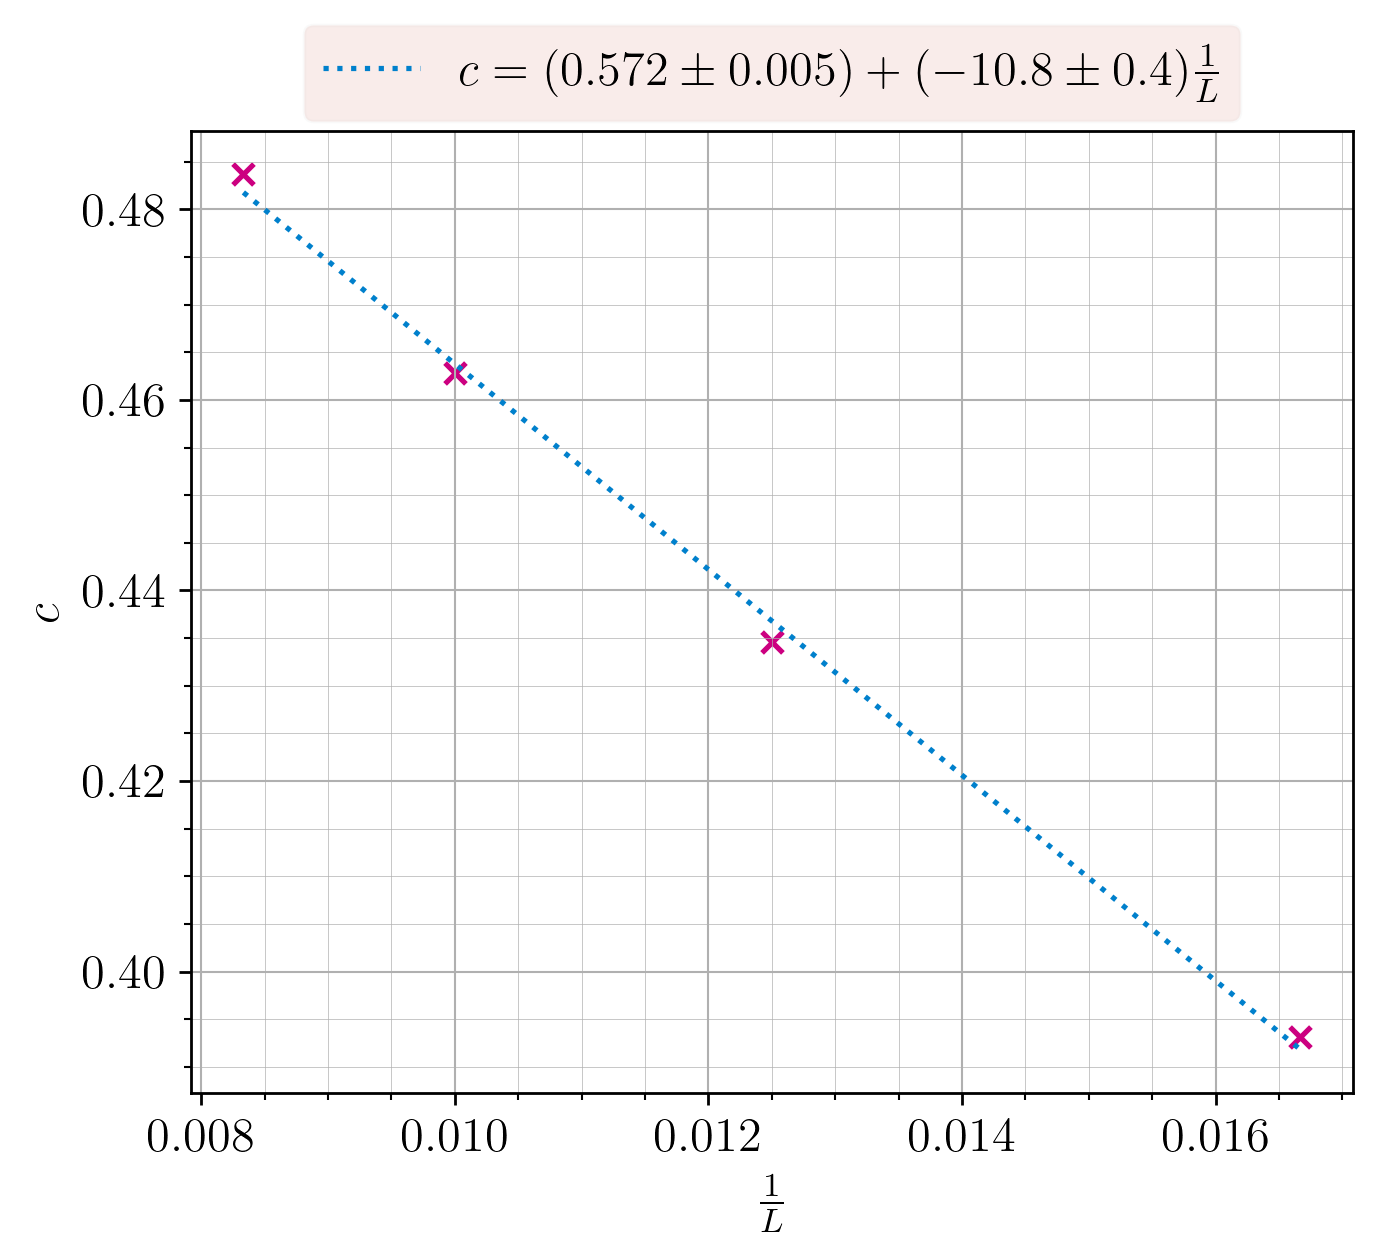
\includegraphics[scale=0.66]{../graphs/entropies/--/100/calabrese_chi=100.0_J=1.0_h=1.0_i=1.0_3=0.856_c=0.0.png}}
		\caption{Extrapolation of the central charge with Cardy-Calabrese formula for $[++]$ OBCs with $h_\text{pin}=-100$ (a): for critical TFI and $\chi=100$. (b): for $\lambda_3/\lambda_I = 0.856$ and $\chi$ sufficiently large to have ground state variance $\sim 10^{-9}$.}
		\label{fig:cPin}
	\end{figure}

	Therefore, another procedure that can be followed to characterize the $\lambda_3/\lambda_I = 0.856$ point is to build conformal towers expected from the CFT describing the corresponding critical point, as well as the ground state energy scaling. To do so, the excitation energies must be retrieved. Following the procedure of \cite{chepiga2017}, the typical behavior of the $10$ first energies found for critical TFI for length $L=70$ is presented on \autoref{fig:energiesTFI} for one complete sweep. It is worth noticing that the Hamiltonian \eqref{eq:TFI} has been rescaled to $\mc H \to \mc H/4$ so that is it now expressed in terms of spin matrices $S^\alpha = \sigma^\alpha/2$. The energies reach a minimum in the middle of the chain, except for the ground state energy, and this value in perfected throughout the sweeps. This minimum will be taken as the value of the excitation energy, again following the work done in \cite{chepiga2017}.

	\begin{figure}[h!]
		\centering
		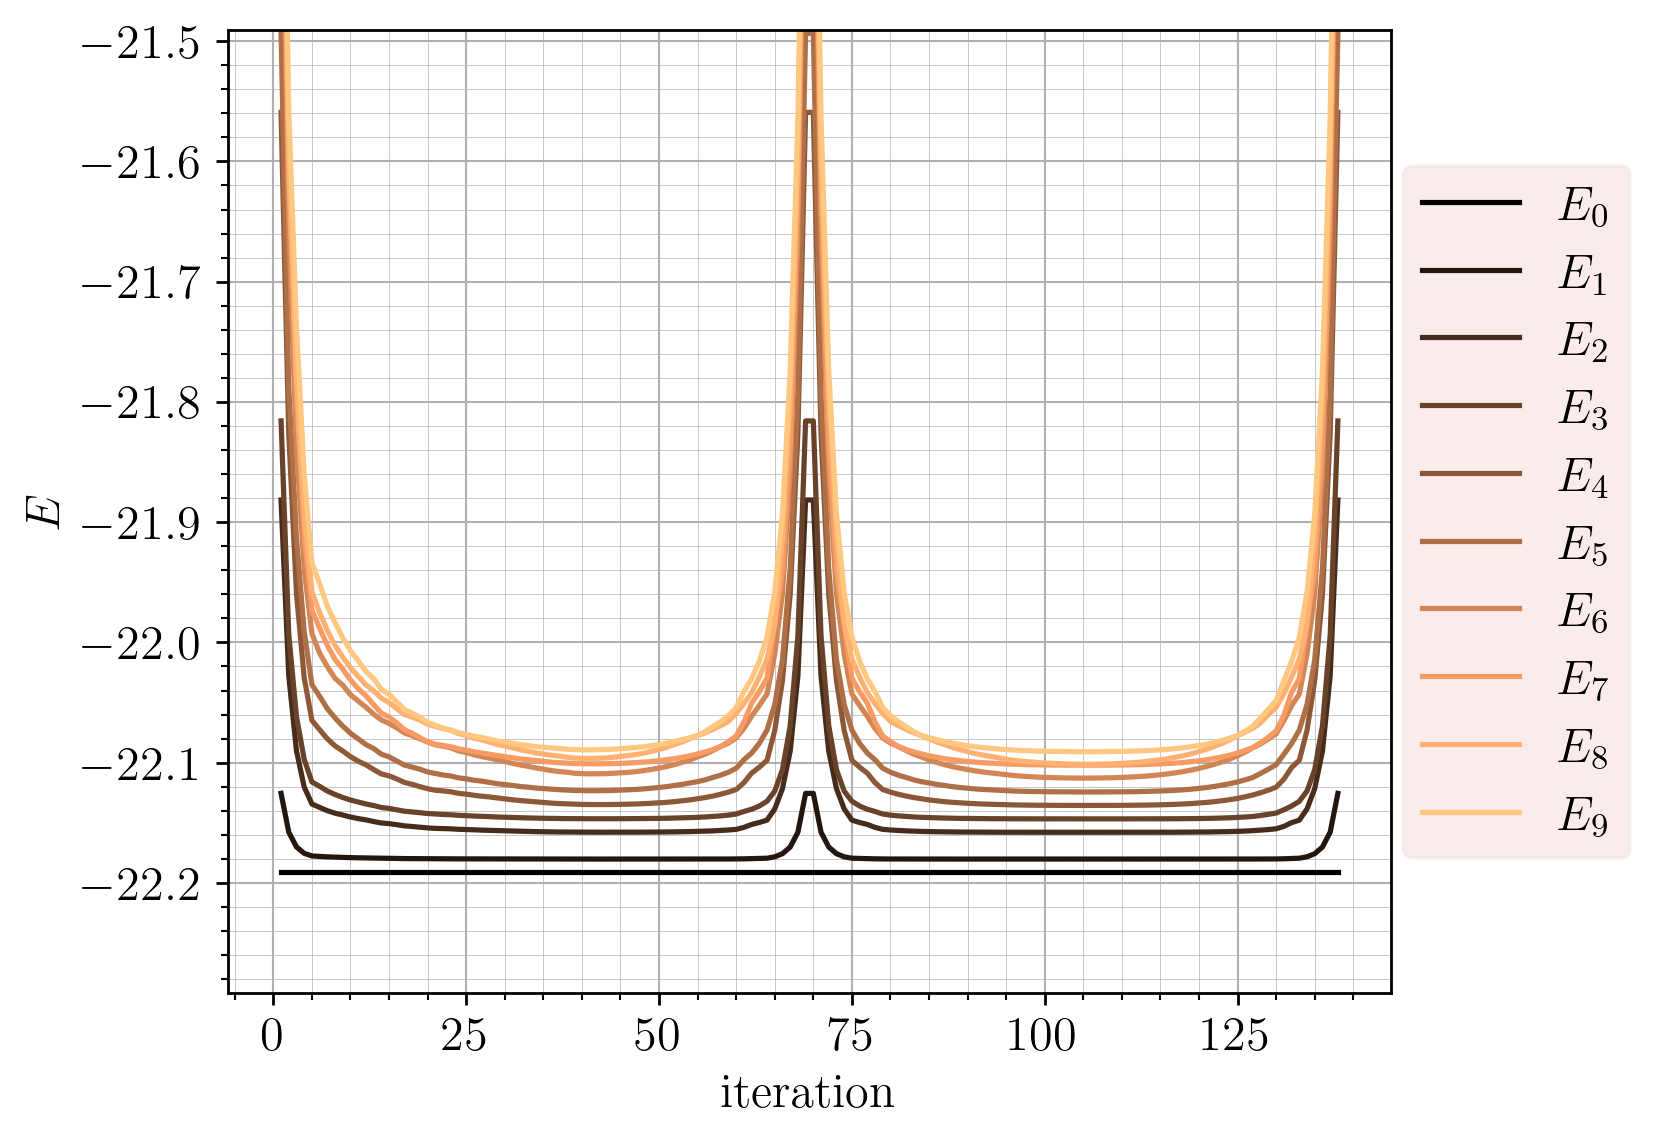
\includegraphics[scale=0.66]{../graphs/conformal/ff/energies_L=70.0_chi=50.0_J=0.25_h=0.25_i=0.5_3=0.0_c=0.0.png}
		\caption{Typical behavior of the lowest-lying energies for one converging sweep of TFI at criticality $J=h$ for one sweep with $L=70$, $\chi=50$ and $[ff]$ OBCs.}
		\label{fig:energiesTFI}
	\end{figure}

	To confirm the correctness of the excited energies $E_n$ -- at least the two first -- the gap of TFI for different values of $h$ is computed and shown on \autoref{fig:gapsTFI} for $L=50$ as well as the extrapolation of the gap in the thermodynamic limit. For $h<J$ the system is ferromagnetic and breaks the $\mathbb Z_2$-symmetry, therefore two degenerate ground states $\ket{+\cdots +}$ and $\ket{-\cdots -}$ are present and thus $|E_1- E_0|$ is expected to vanish. The gap in this ordered phase is expected to be $2|J|(1-|h|)$ \cite{pfeuty1970} and is exactly the value found for $|E_2-E_0|$, knowing that $J=1$ here. Moreover, for $h>J$ the systems is paramagnetic and has a non-degenerate ground state with a gap $2|J|(|h|-1)$. Finally, for $J=h$, the systems goes under a phase transition and expected to have a continuous spectrum. The gap is then observed to close exponentially fast in $1/L$.

	\begin{figure}[h!]
		\hspace{-0.5cm}
		\subfloat[]{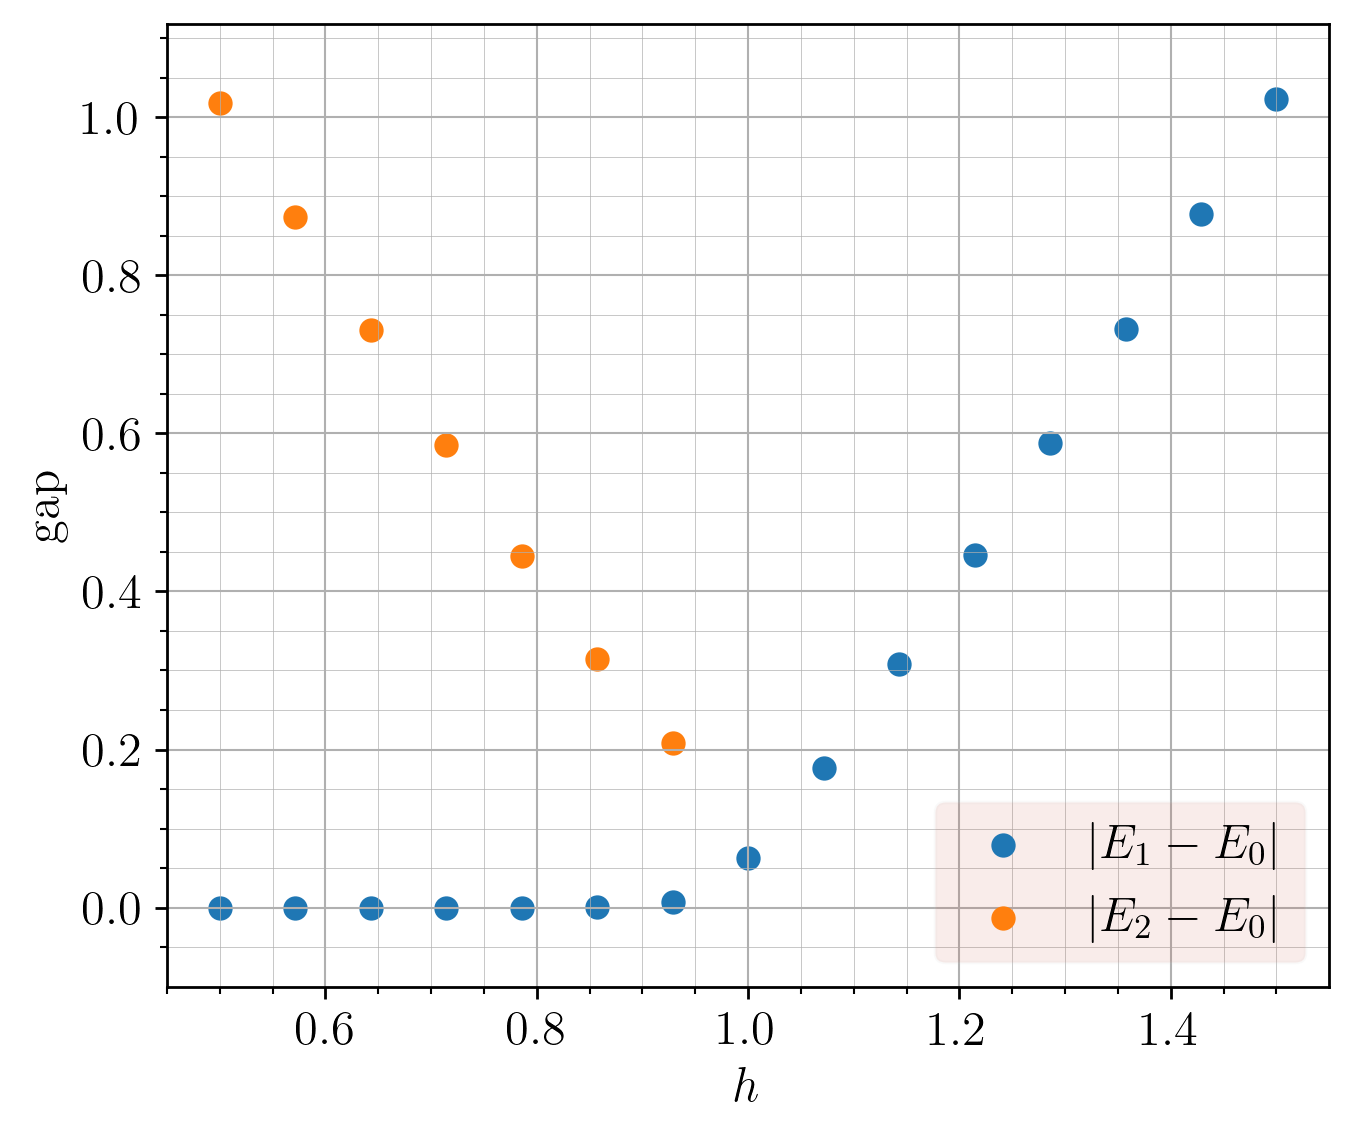
\includegraphics[scale=0.66]{../graphs/transition/ff/gap_L=50_chi=50.0_J=1.0_i=0.5_3=0.0_c=0.0.png}}\quad
		\subfloat[]{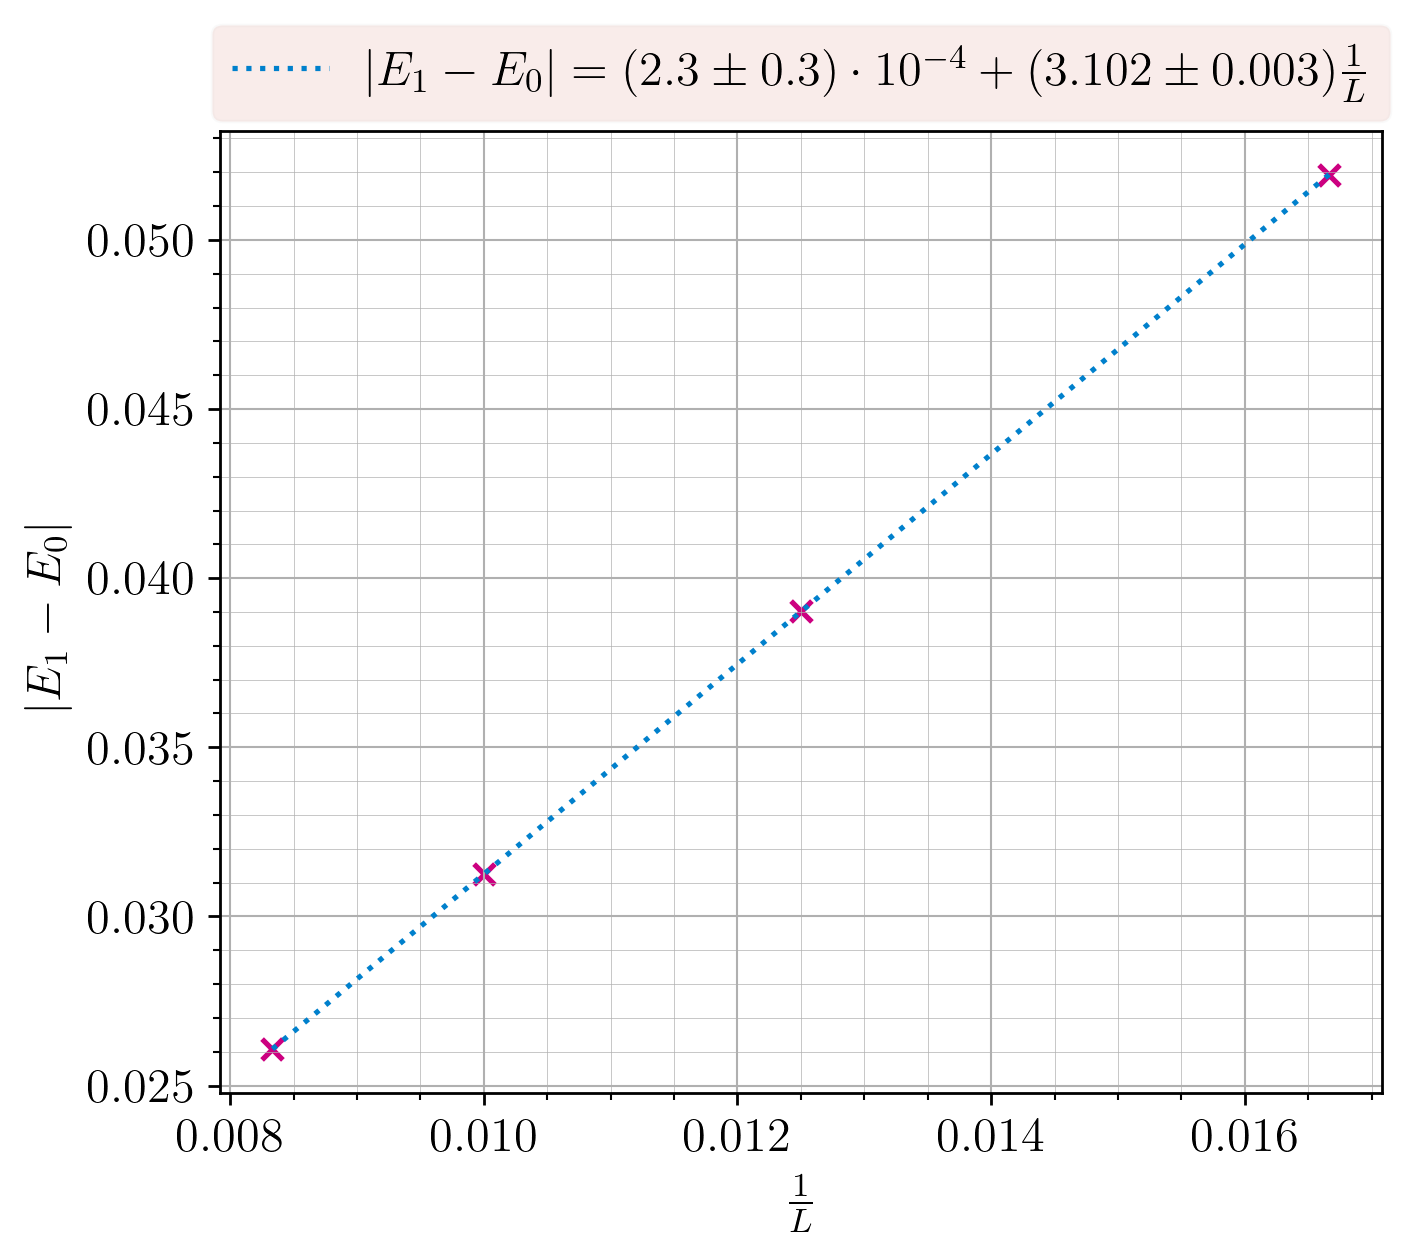
\includegraphics[scale=0.66]{../graphs/gaps/ff/gap_chi=200.0_J=1.0_h=1.0_i=1.0_3=0.0_c=0.0.png}}
		\caption{TFI with $[ff]$ OBCs. (a): Gap between first two non-degenerate energies of TFI for $L=50$ and $\chi=50$ as the field $h$ is varied. (b): Extrapolation of the gap at criticality $J=h$ for $\chi=200$.}
		\label{fig:gapsTFI}
	\end{figure}

	The energy scaling of the ground state has been expressed in \cite{affleck1986} and can be written \cite{blote1986, lassig1991}, once again following \cite{chepiga2017},
	\be E_0 = \varepsilon_0 L + \frac{\pi v}{L}\left[\Delta -\frac{1}{48}\right] + \varepsilon_1 \label{eq:gsScaling} \ee
	where $v = \frac 1 2$ for Ising CFT \cite{affleck1986}, $\varepsilon_0, \varepsilon_1$ non-universal fitting parameters to account for finite size effect and $\Delta$ the conformal dimension of the primary field of the Ising CFT, or the minimum conformal dimension if there is a superposition of several towers. For Ising CFT, there are $3$ fields realized via some OBCs and are given in \autoref{tab:isingConfDim} \cite{cardy1986, cardy1989, francesco1997}. Moreover, the $[ff]$ condition is realized via superposition of $\one$ and $\varepsilon$.

	\begin{table}[h!]
		\centering
		\renewcommand{\arraystretch}{1.3}
		\begin{tabular}{ccc}
			Operator & Dimension & Realization \\
			\hline
			$\one$ & $0$ & $[++]\ [--]$ \\
			$\varepsilon$ & $\frac 1 2$ & $[+-]\ [-+]$ \\
			$\sigma$ & $\frac{1}{16}$ & $[f-]\ [f+]\ [-f]\ [+f]$ \\
			\hline
		\end{tabular}
		\caption{Different CFT operators realized with corresponding boundary conditions and their dimension, used for the construction of the conformal towers..}
		\label{tab:isingConfDim}
	\end{table}

	Therefore, the scaling of ground state energy of critical TFI is presented on \autoref{fig:gsSalingTFI}, where only one realization of each operator is shown and $v\sim 1/2$ quite precise for all of them. Each time, the ground state energy if fitted with \eqref{eq:gsScaling} to find $\varepsilon_0$ and $\varepsilon_1$, and where $v$ can also be computed. Then a linear regression is performed of $\frac{E_0 - \varepsilon_1}{L} - \varepsilon_0$ against $1/L^2$ for a neat view and where the intercept is found to be negligible, as wanted.

	\begin{figure}[h!]
		\hspace{-0.5cm}
		\begin{minipage}{\linewidth}
			\subfloat[]{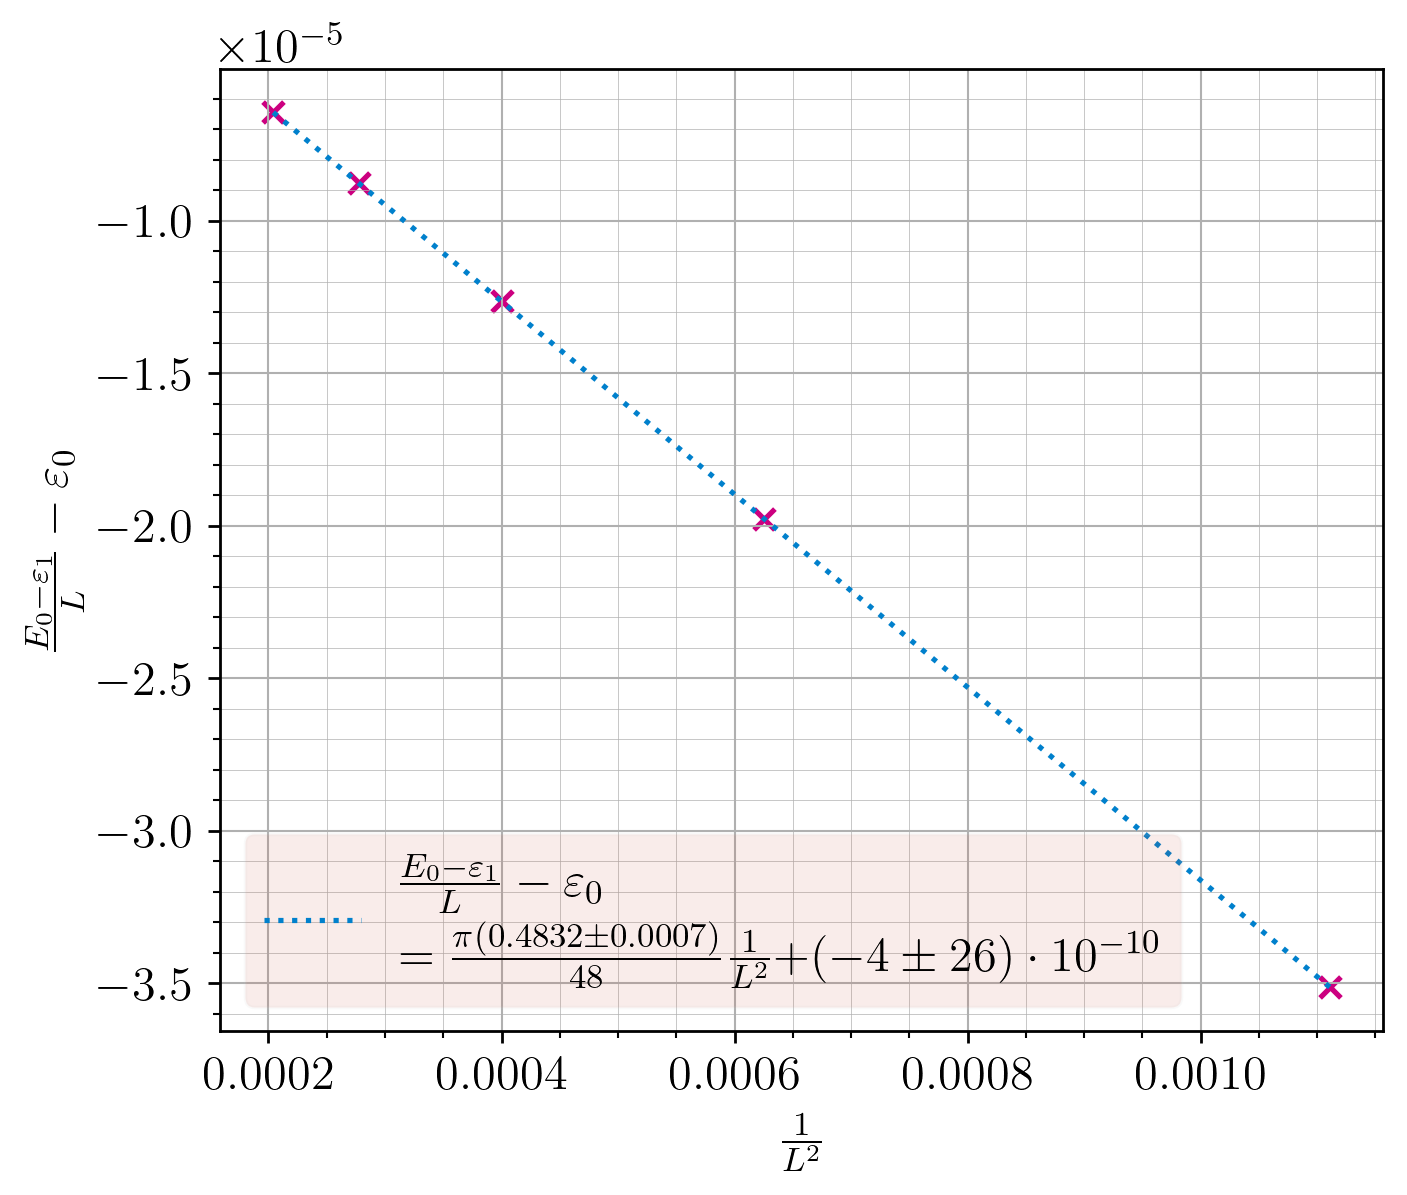
\includegraphics[scale=0.66]{../graphs/conformal/ff/gs_chi=50.0_J=0.25_h=0.25_i=0.5_3=0.0_c=0.0.png}}\
			\subfloat[]{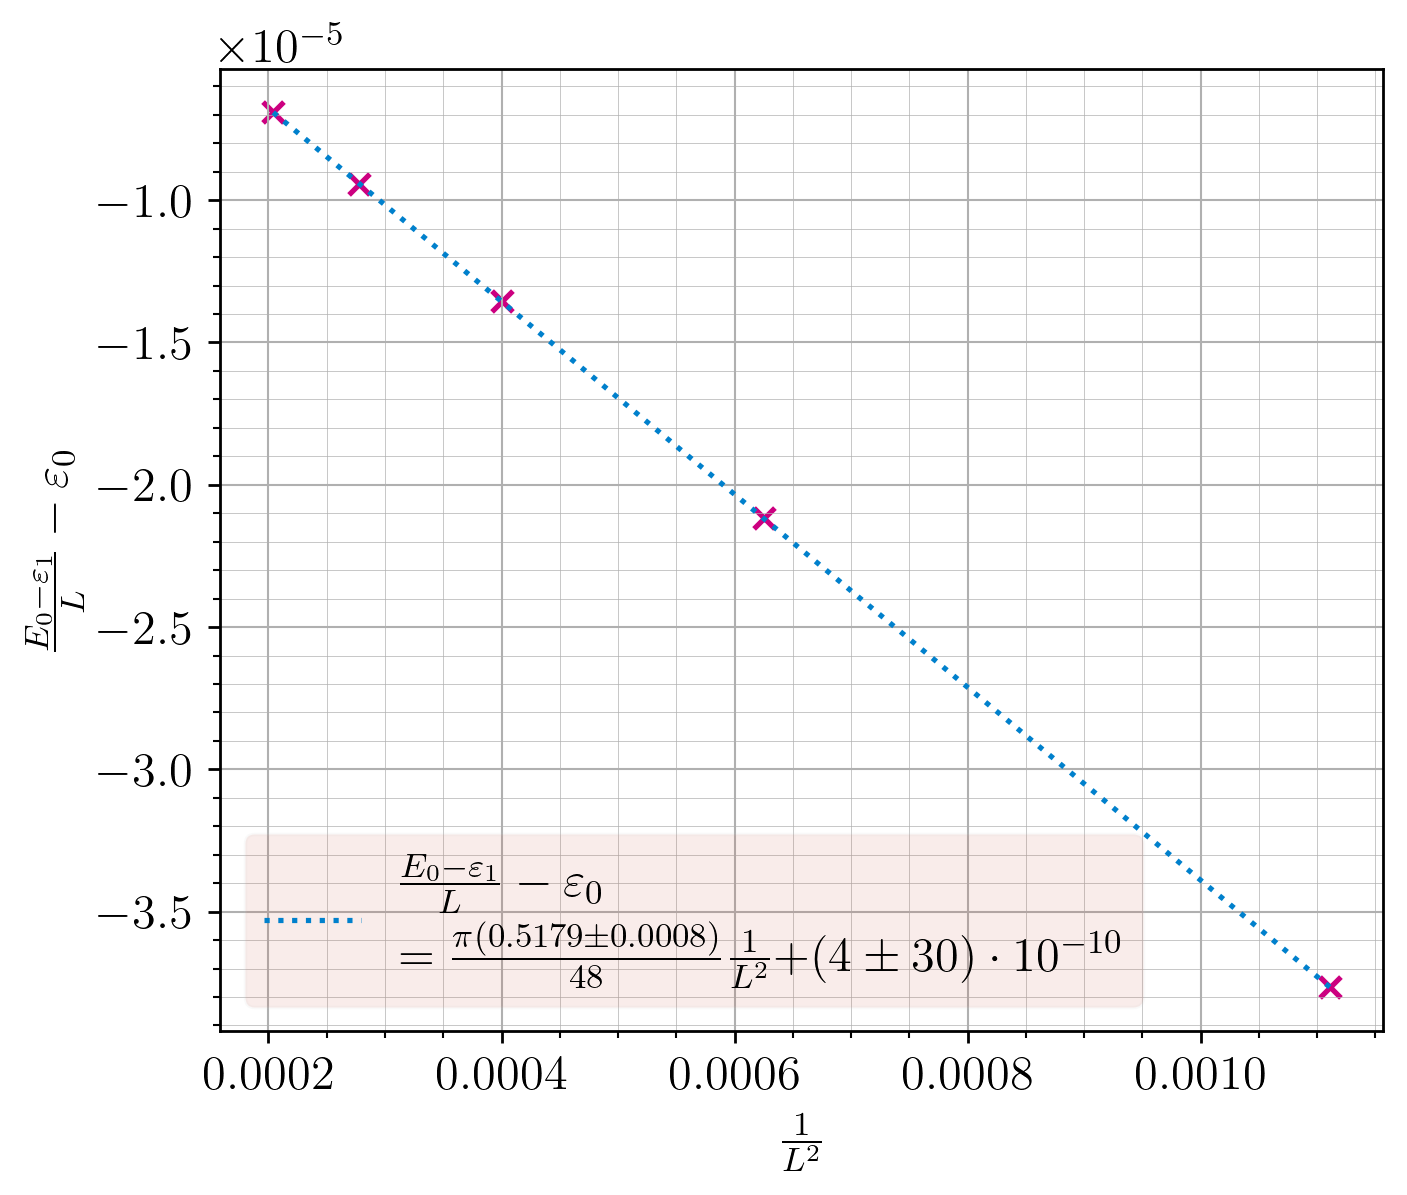
\includegraphics[scale=0.66]{../graphs/conformal/100/--/gs_chi=50.0_J=0.25_h=0.25_i=0.5_3=0.0_c=0.0.png}}
		\end{minipage}

		\hspace{-0.5cm}
		\begin{minipage}{\linewidth}
			\subfloat[]{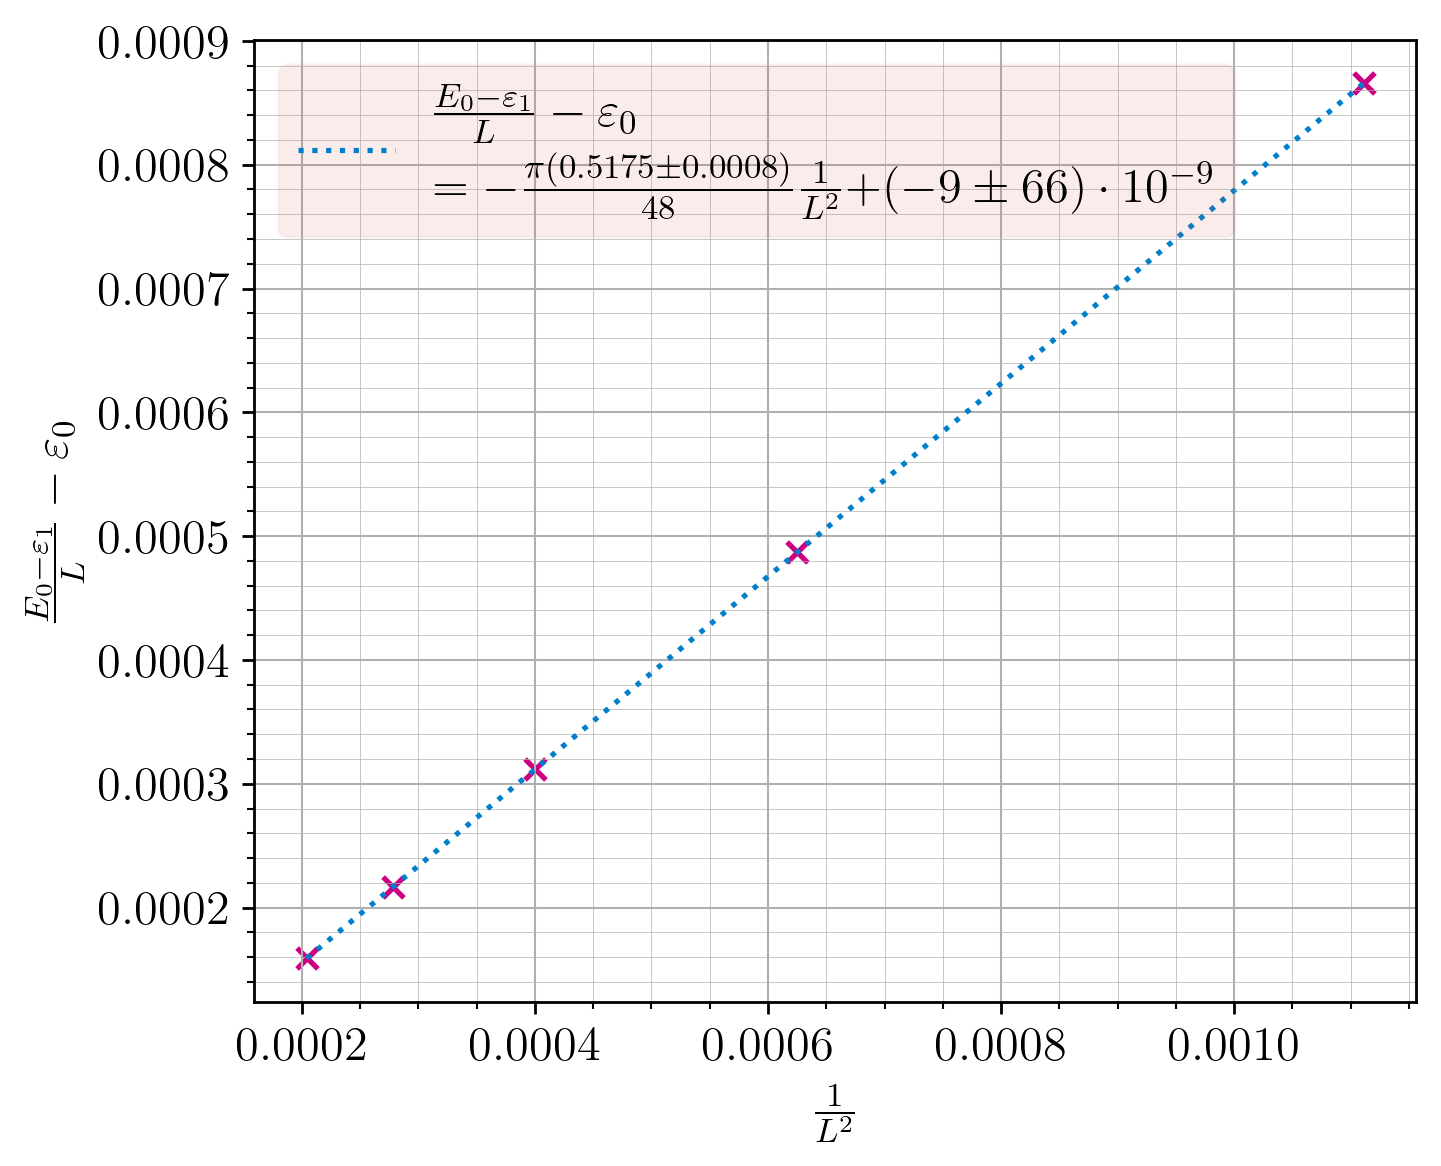
\includegraphics[scale=0.66]{../graphs/conformal/100/+-/gs_chi=50.0_J=0.25_h=0.25_i=0.5_3=0.0_c=0.0.png}}\
			\subfloat[]{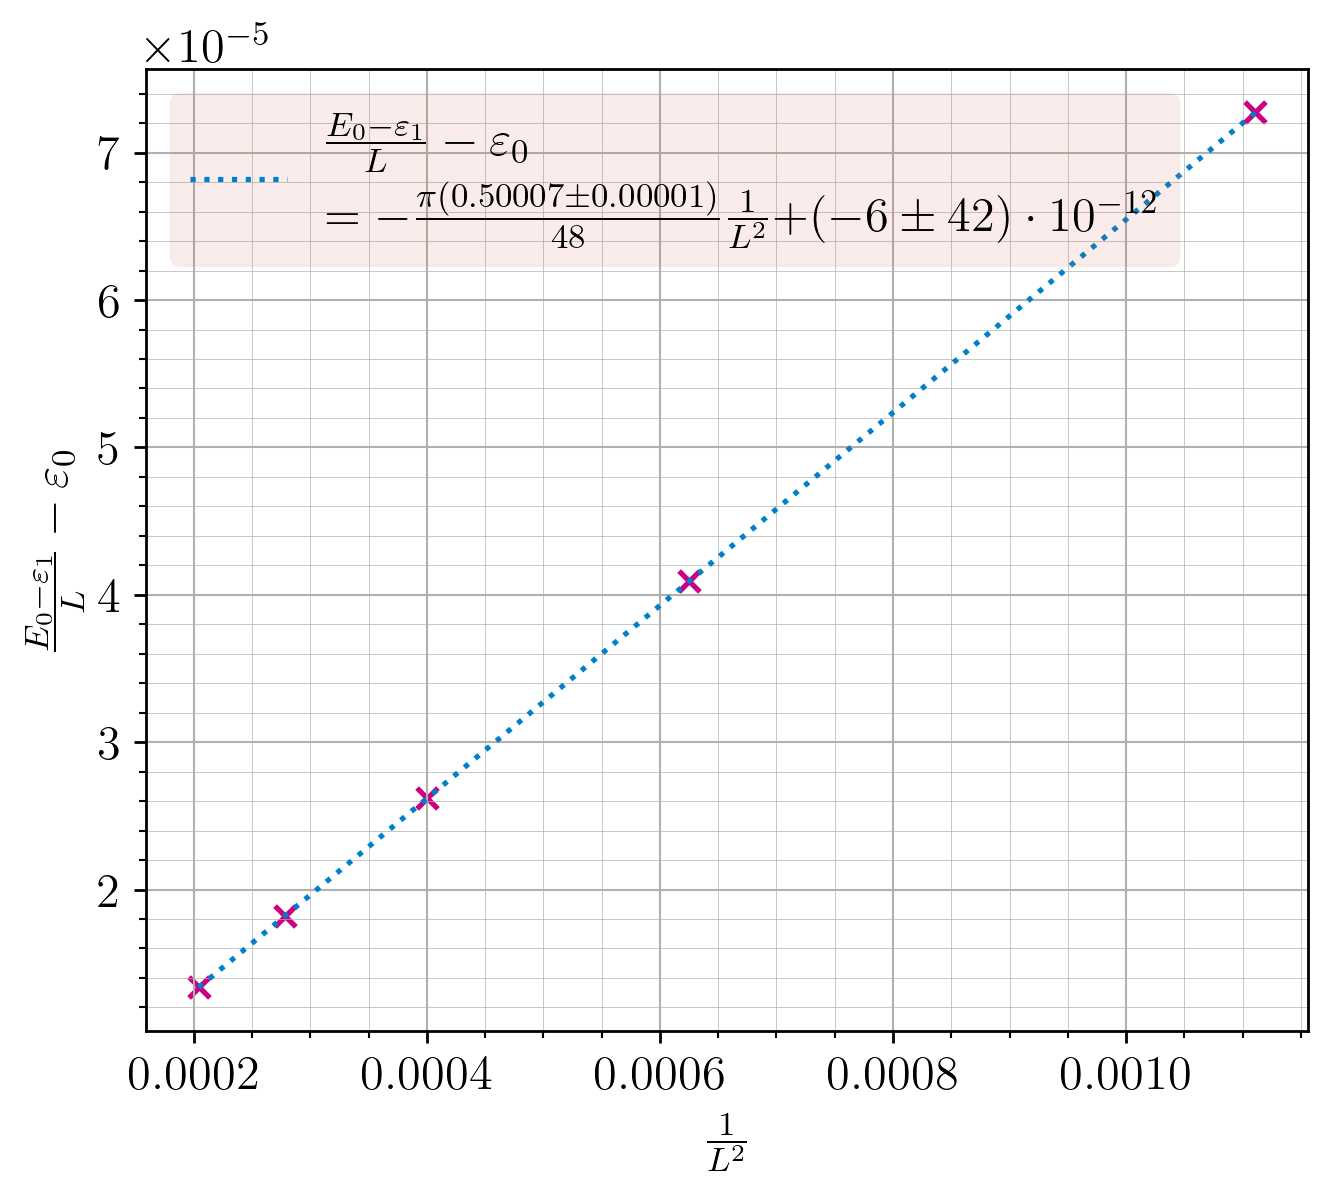
\includegraphics[scale=0.66]{../graphs/conformal/100/f+/gs_chi=50.0_J=0.25_h=0.25_i=0.5_3=0.0_c=0.0.png}}
		\end{minipage}
		\caption{Ground state energy scaling for critical TFI and $\chi=50$ for (a): $[ff]$ OBCs. (b): $[++]$ OBCs. (c): $[-+]$ OBCs. (d): $[f-]$ OBCs. The coefficient in front of $1/L^2$ depends on the conformal dimension of the operator realizing the OBCs, or on the minimum of them if the OBCs are a superposition of several operators. If not free, each edge has pinning magnitude $|h_\text{pin}|=100$.}
		\label{fig:gsSalingTFI}
	\end{figure}

	The conformal towers are finally observed on \autoref{fig:towersTFI} with $10$ energies computed, again following \cite{chepiga2017}. Each excitation has a certain multiplicity taken from the characters of the irreducible representations of the model \cite{cardy1986, cardy1989, francesco1997} and correspond to the one found for each tower for Ising CFT. The characters are explicitly described in \cite{chepiga2017}. In order in them for each operator gives a line in the figure. It can be seen that they agree very well with the data with the multiplicities -- the coefficient of each order -- found at each level agreeing as well. It has been therefore shown that the way to compute the excitation energies is correct, at least for TFI.

	The construction of the conformal towers for TCI CFT for the point $\lambda_3/\lambda_I$ was wanted to be made, to characterize this point with another way than the central charge  which compellingly seemed to be cursed for OBCs. Moreover, the PBCs could have resolved this problem of central charge, but unfortunately a small and well hidden mistake had been made in the construction of the PBCS MPO for \eqref{eq:OF} and the use of these boundary conditions was about to be dropped. However, being a very beginner, finding the expansion of the characters correctly as well as the realization of the primary field of TCI CFT via some boundary conditions was hard. Some references have been found \cite{affleck2000, belavin1984, cardy1986, cardy1989, friedan1985, friedan1984, lassig1991, qiu1986}, but in the meantime, the PBCs MPO problem has been resolved so the works moved on the use of these PBCs as in \cite{obrien2018}.

	\begin{figure}[h!]
		\hspace{-0.5cm}
		\begin{minipage}{\linewidth}
			\subfloat[]{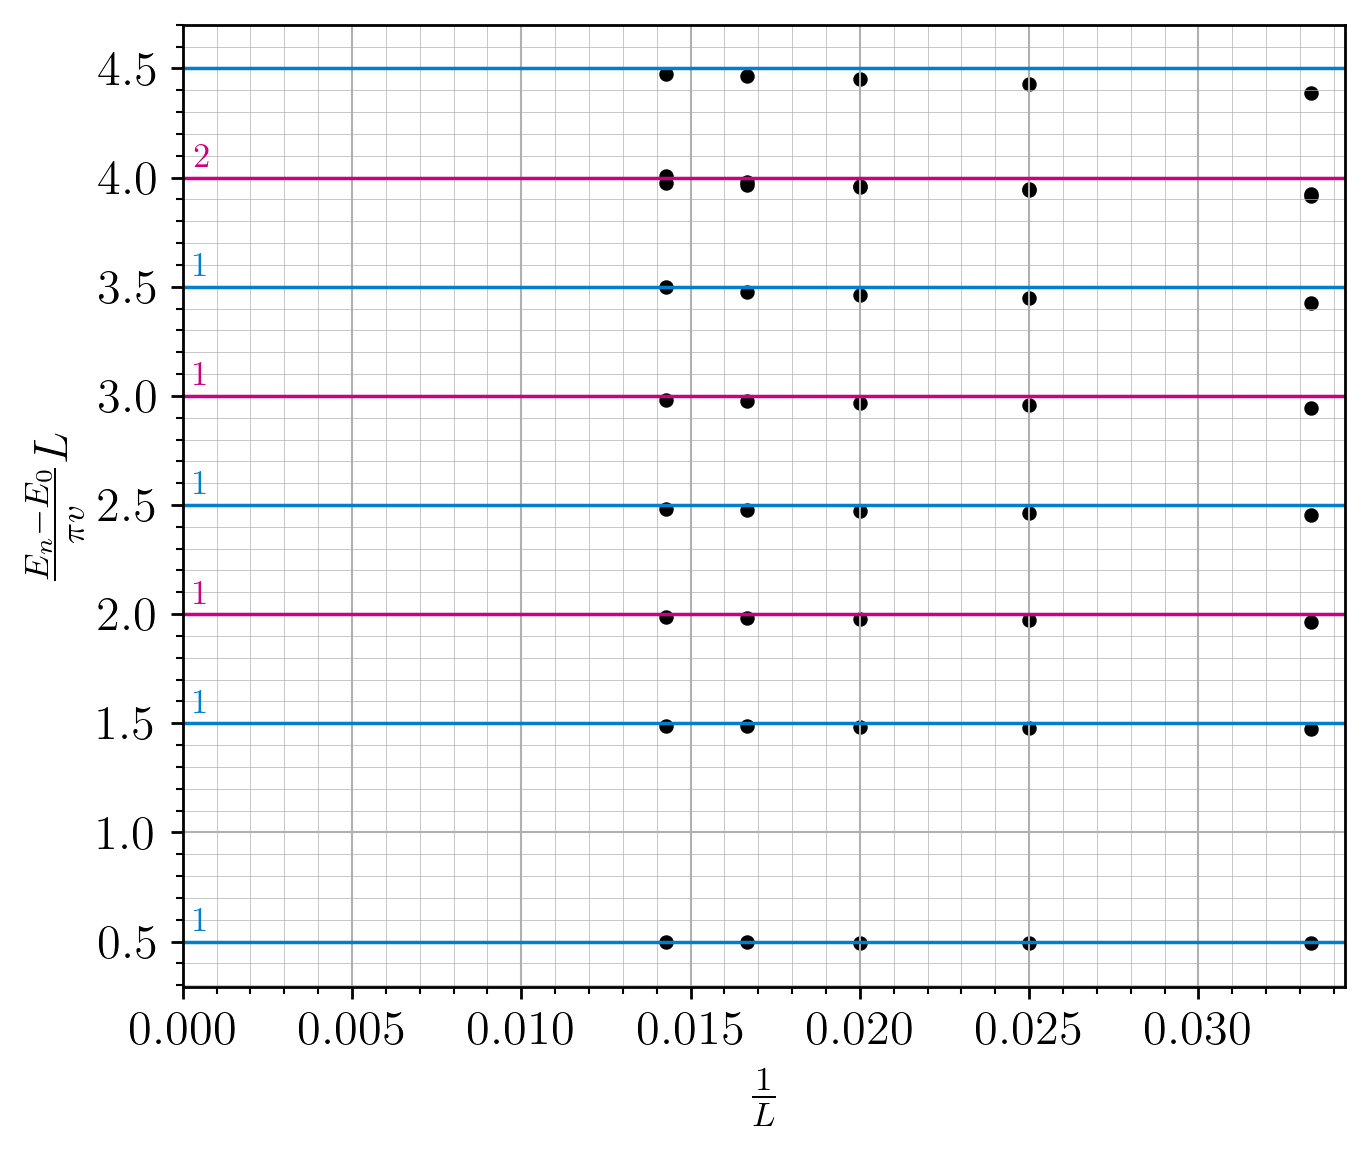
\includegraphics[scale=0.66]{../graphs/conformal/ff/towers_chi=50.0_J=0.25_h=0.25_i=0.5_3=0.0_c=0.0.png}}\
			\subfloat[]{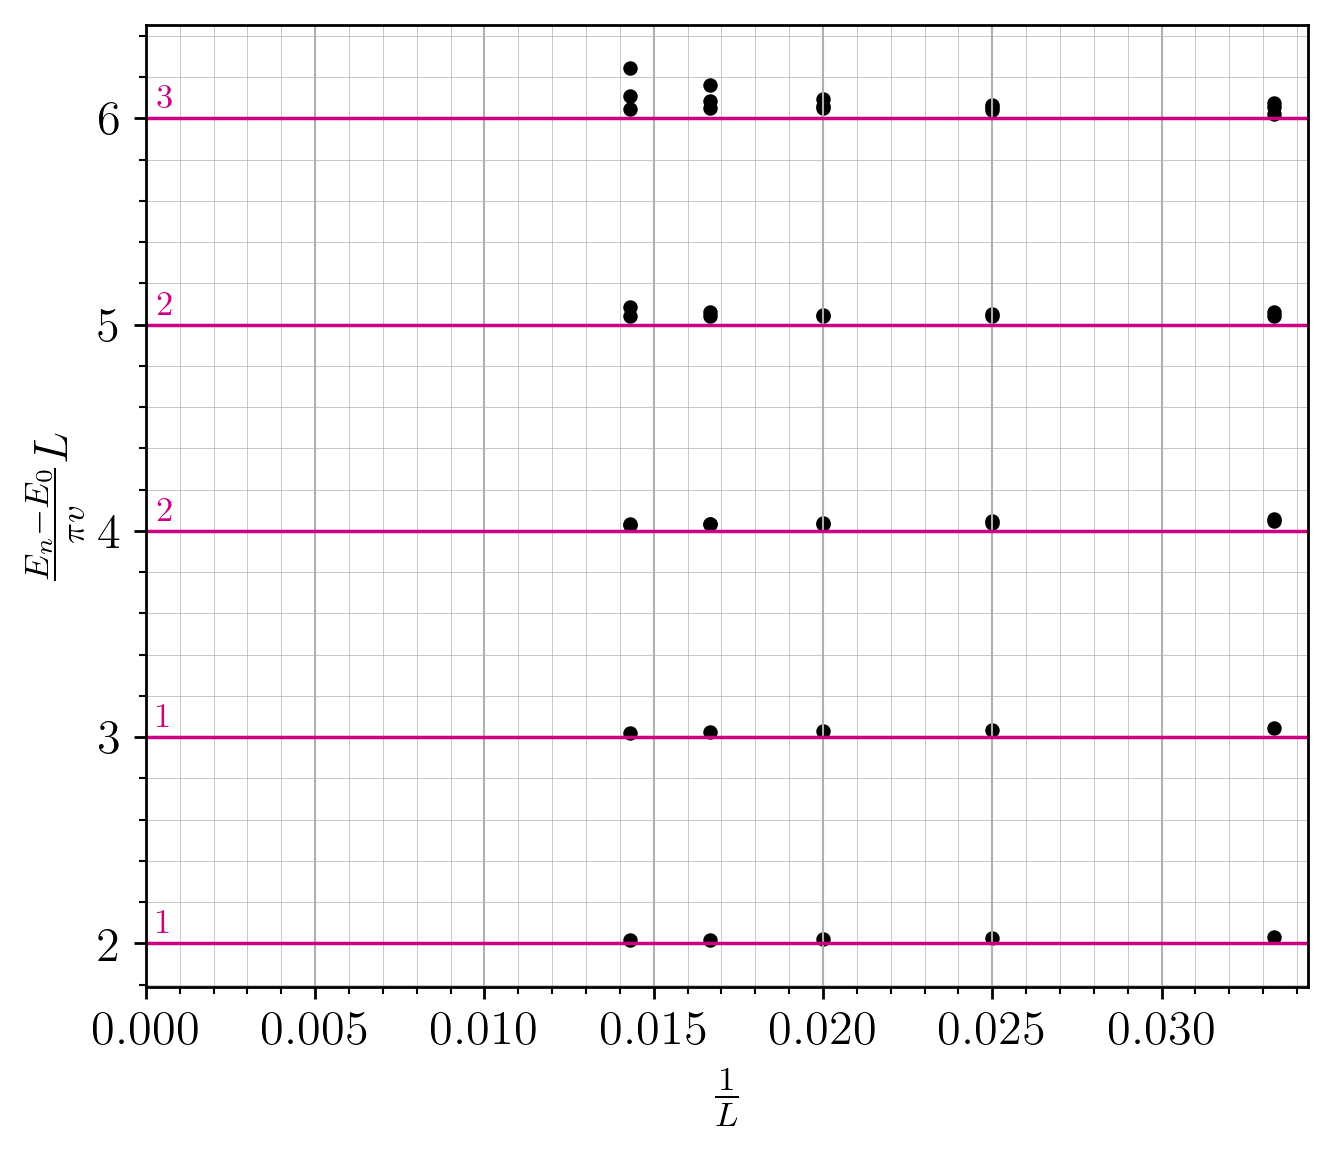
\includegraphics[scale=0.66]{../graphs/conformal/100/--/towers_chi=50.0_J=0.25_h=0.25_i=0.5_3=0.0_c=0.0.png}}
		\end{minipage}

		\hspace{-0.5cm}
		\begin{minipage}{\linewidth}
			\subfloat[]{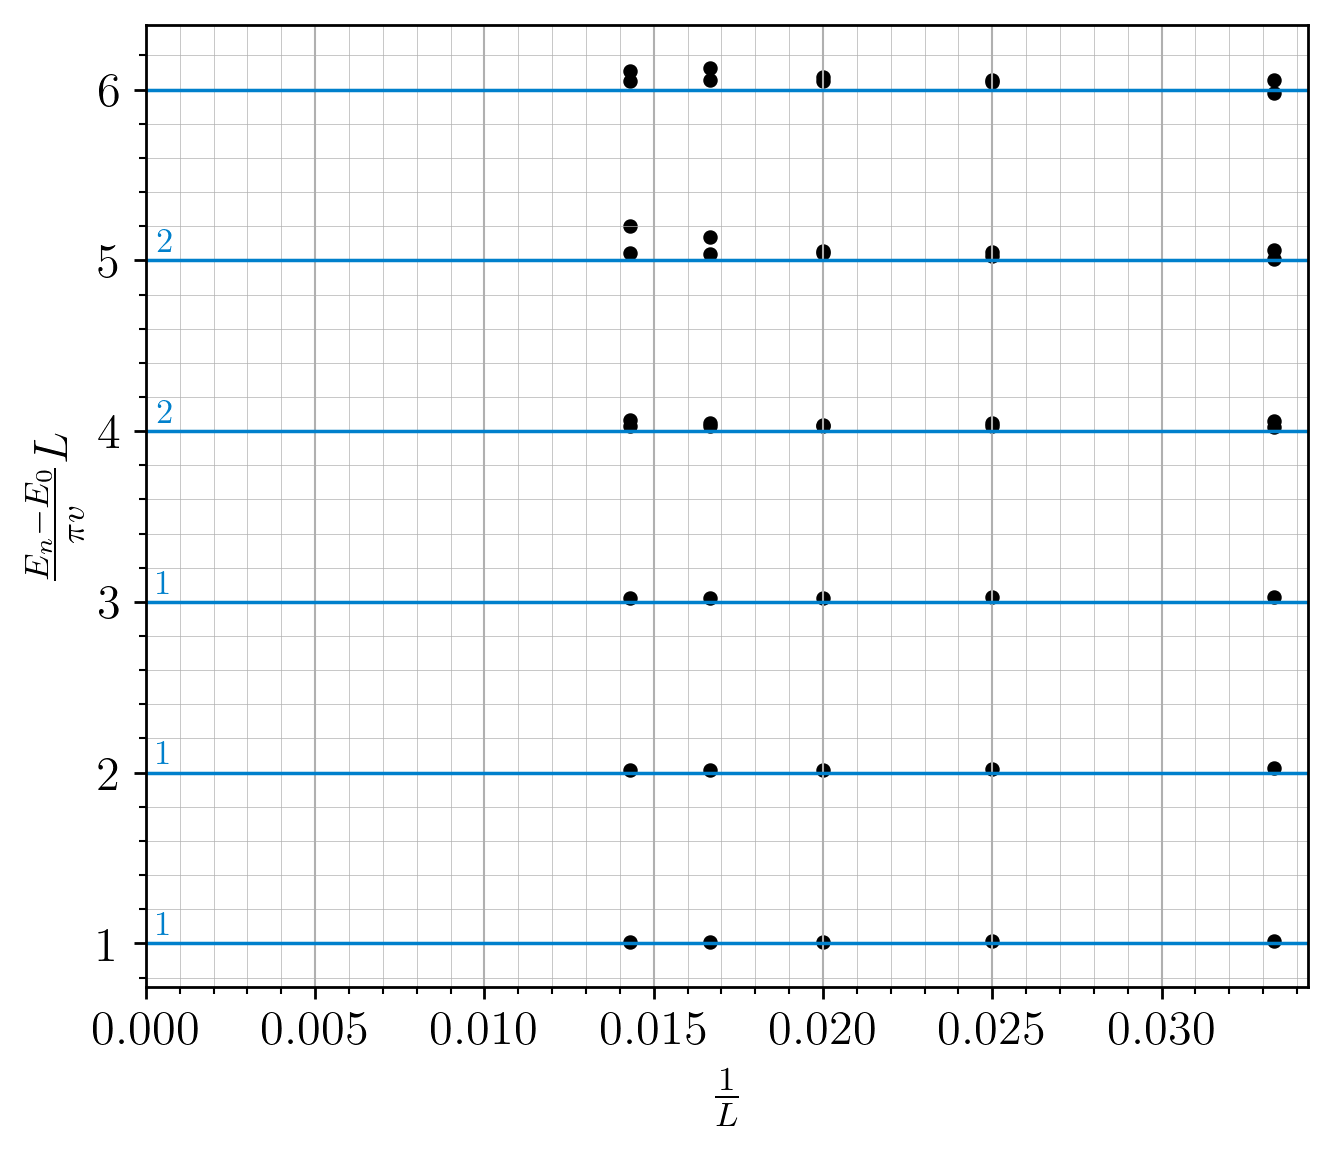
\includegraphics[scale=0.66]{../graphs/conformal/100/+-/towers_chi=50.0_J=0.25_h=0.25_i=0.5_3=0.0_c=0.0.png}}\
			\subfloat[]{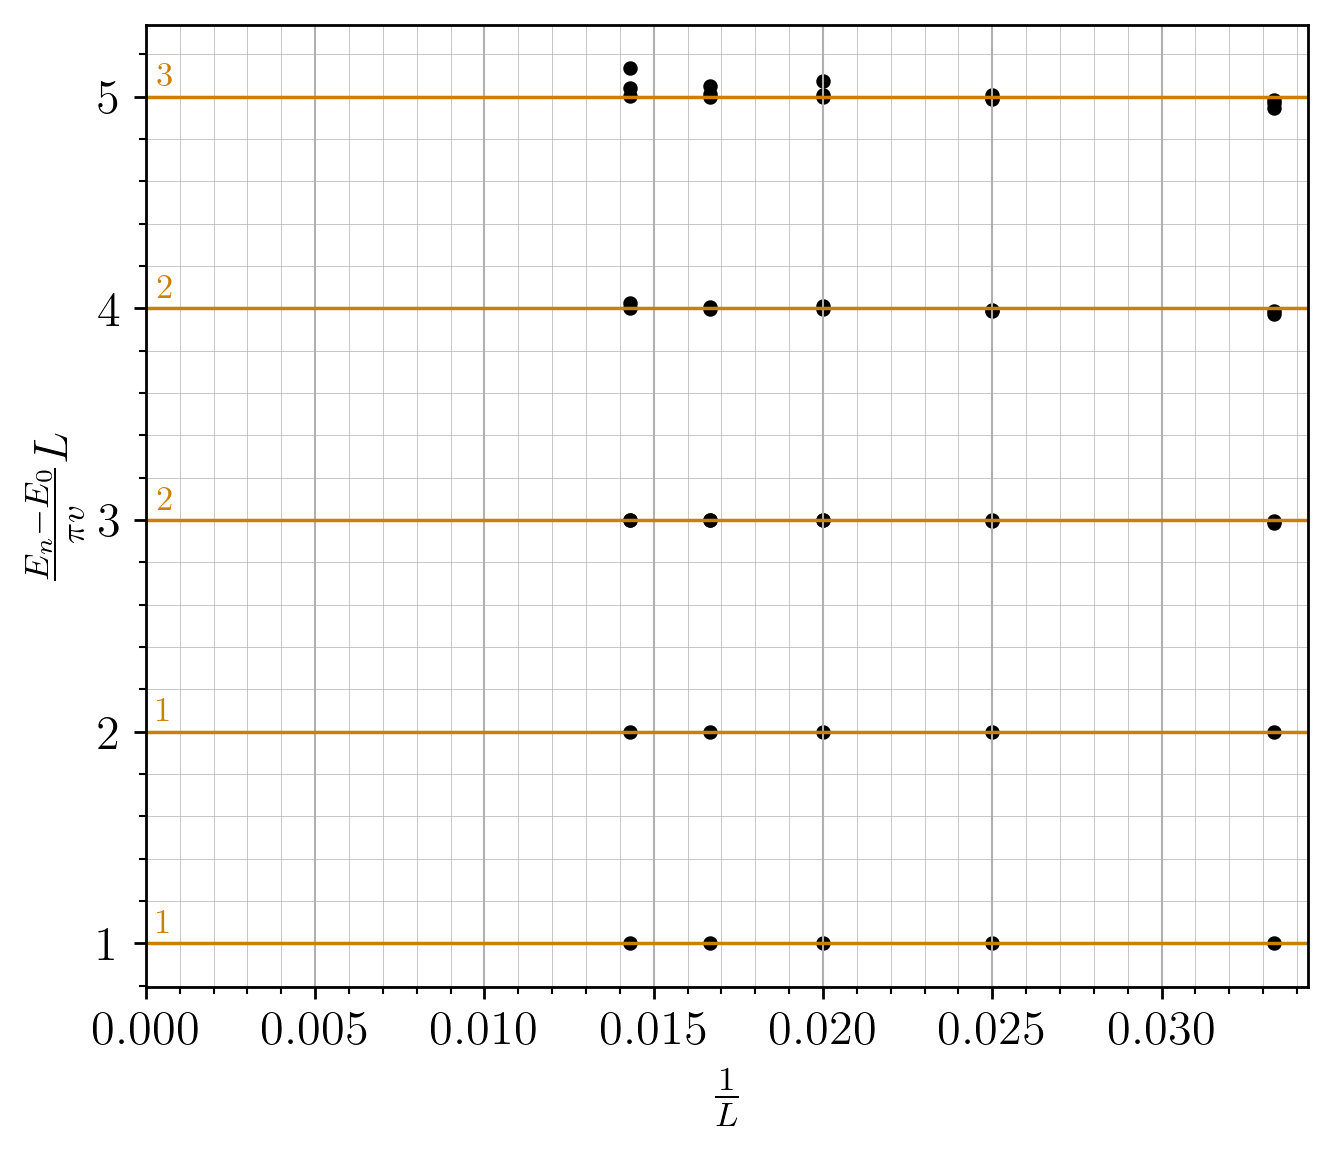
\includegraphics[scale=0.66]{../graphs/conformal/100/f+/towers_chi=50.0_J=0.25_h=0.25_i=0.5_3=0.0_c=0.0.png}}
		\end{minipage}
		\caption{Conformal tower obtained for critical TFI and $\chi=50$ for for (a): $[ff]$ OBCs. (b): $[++]$ OBCs. (c): $[-+]$ OBCs. (d): $[f-]$ OBCs. Black dots represent data. Lines represent predictions from CFT and the numbers the degeneracy obtained for each level. Magenta is for $\mathbb{1}$, cyan for $\varepsilon$ and yellow for $\sigma$. If not free, each edge has pinning magnitude $|h_\text{pin}|=100$. Notice that $v=1/2$ here coming from Ising CFT.}
		\label{fig:towersTFI}
	\end{figure}

	Now that the PBCs work -- at least the correct ground state energy was recovered -- the central charge can be computed, this time using \eqref{eq:cardyPBCs}. It is recovered by extrapolating in $1/L^2$, as it is usually done \cite{milsted2017}, for both critical TFI and OF at $\lambda_3/\lambda_I=0.856$ on \autoref{fig:cPBCs}. A low variance is very difficult to obtain for reasonable bond dimensions, especially for \eqref{eq:OF}, then $\chi$ was chosen each time to reach a descent variance of $\sim 10^{-4}$. Also, it can be observed for critical TFI the extrapolation of $c$ is precise to $10^{-5}$ and even the individual values are in the scale of $10^{-5}$ for quite small lengths between $40$ and $70$. A worse precision is obtained for $\lambda_3/\lambda_I=0.856$ for each individual data and the extrapolation but it is still very acceptable and goes to $c=0.699586\pm0.000008$ being close up to $\sim 10^{-3}$ to $0.7$ expected for TCI CFT. It seems the PBCs completely resolved the problem of the central charge, and it can be conclude, even if no much compelling evidence for now, that since the central charge of the OF model at $\lambda_3/\lambda_I=0.856$ is the one of TCI, this point is effectively in the TCI CFT. Further computation will be made to completely characterize it.

	\begin{figure}[h!]
		\hspace{-0.4cm}
		\subfloat[]{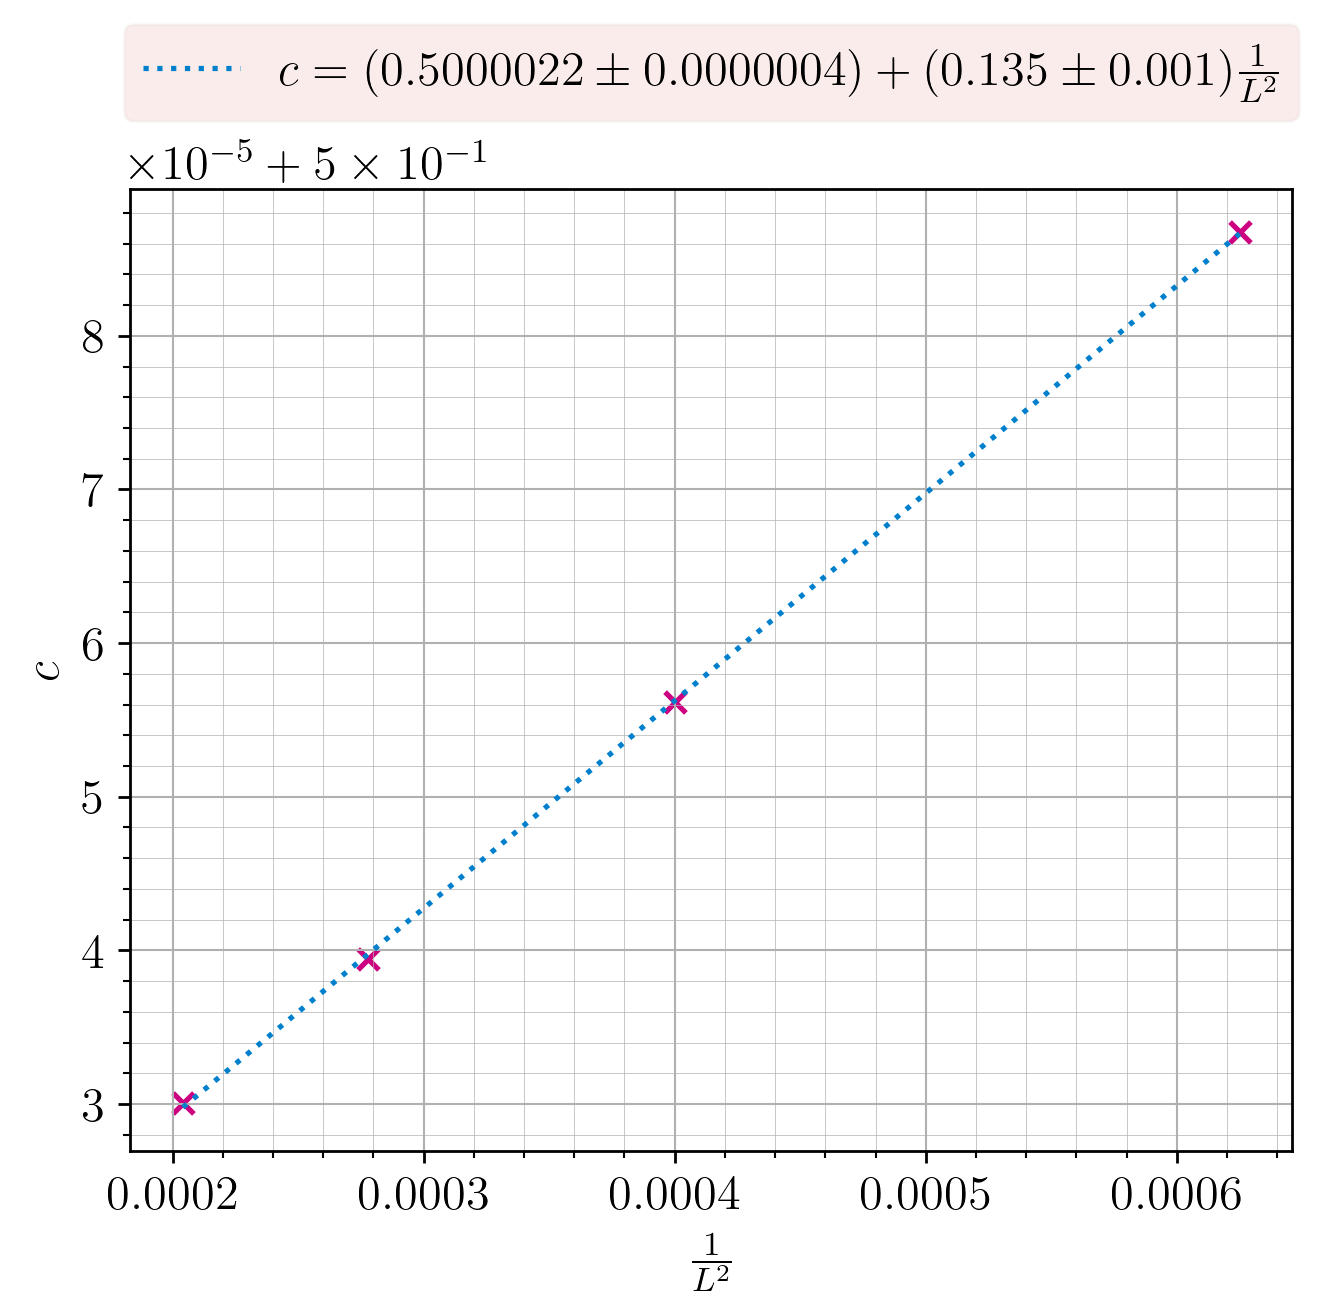
\includegraphics[scale=0.66]{../graphs/entropies/pbc/10-9/calabrese_J=1.0_h=1.0_i=1.0_3=0.0_c=0.0.png}}\quad
		\subfloat[]{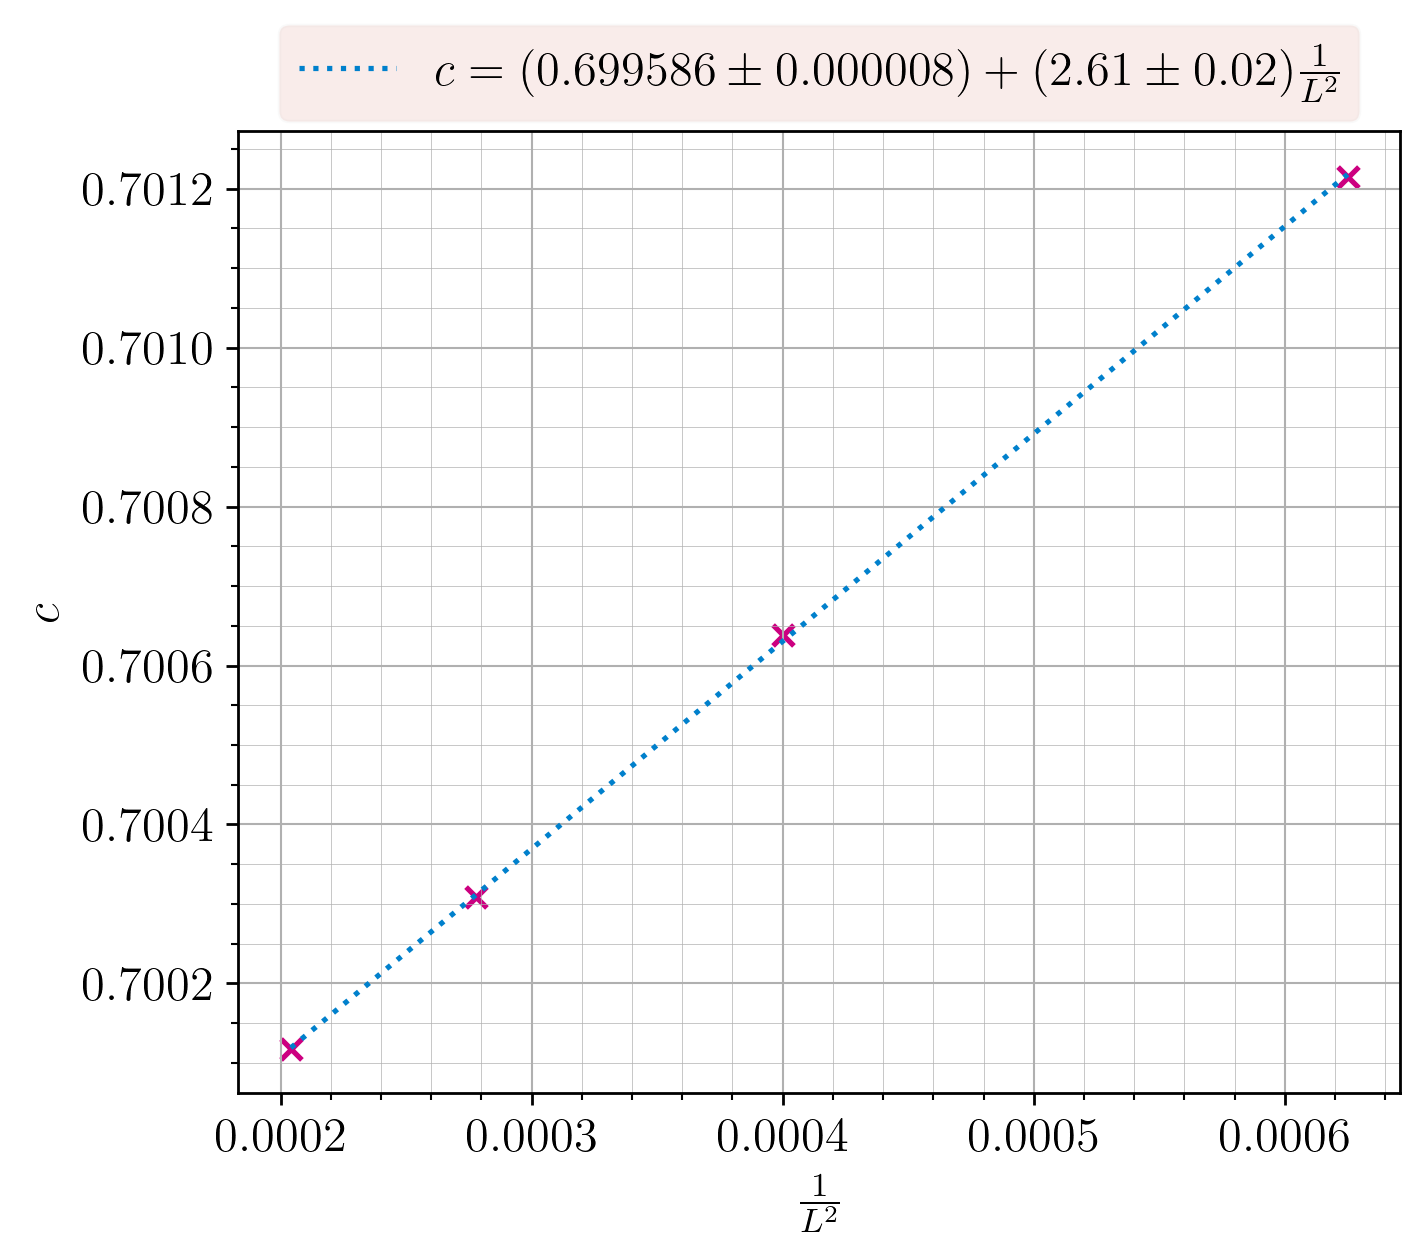
\includegraphics[scale=0.66]{../graphs/entropies/pbc/10-4/calabrese_J=1.0_h=1.0_i=1.0_3=0.856_c=0.0.png}}
		\caption{Extrapolation of the central charge with Cardy-Calabrese formula with PBCs (a): for critical TFI with ground state variance $\sim 10^{-9}$. (b): for $\lambda_3/\lambda_I = 0.856$ with ground state variance $\sim 10^{-4}$.}
		\label{fig:cPBCs}
	\end{figure}

	On \autoref{fig:phasePBCs}, results from \autoref{fig:phaseOBCs} are repeated with PBCs as the ratio $\lambda_3/\lambda_I=0.856$ is varied the see how the central charge behave along this line. This time, the main observation is that the central charge does not reach a maximum before decreasing for $0.7\leq\lambda_3/\lambda_I\leq0.85$, but it monotonically decreasing towards $c\sim 0.5$. The point $\lambda_3/\lambda_I=0.856$ seems to stay at the value $c \sim 0.7$ in $1/L^2$. Consequently, PBCs seem to have resolved the problem of the OBCs.

	\begin{figure}[h!]
		\centering
		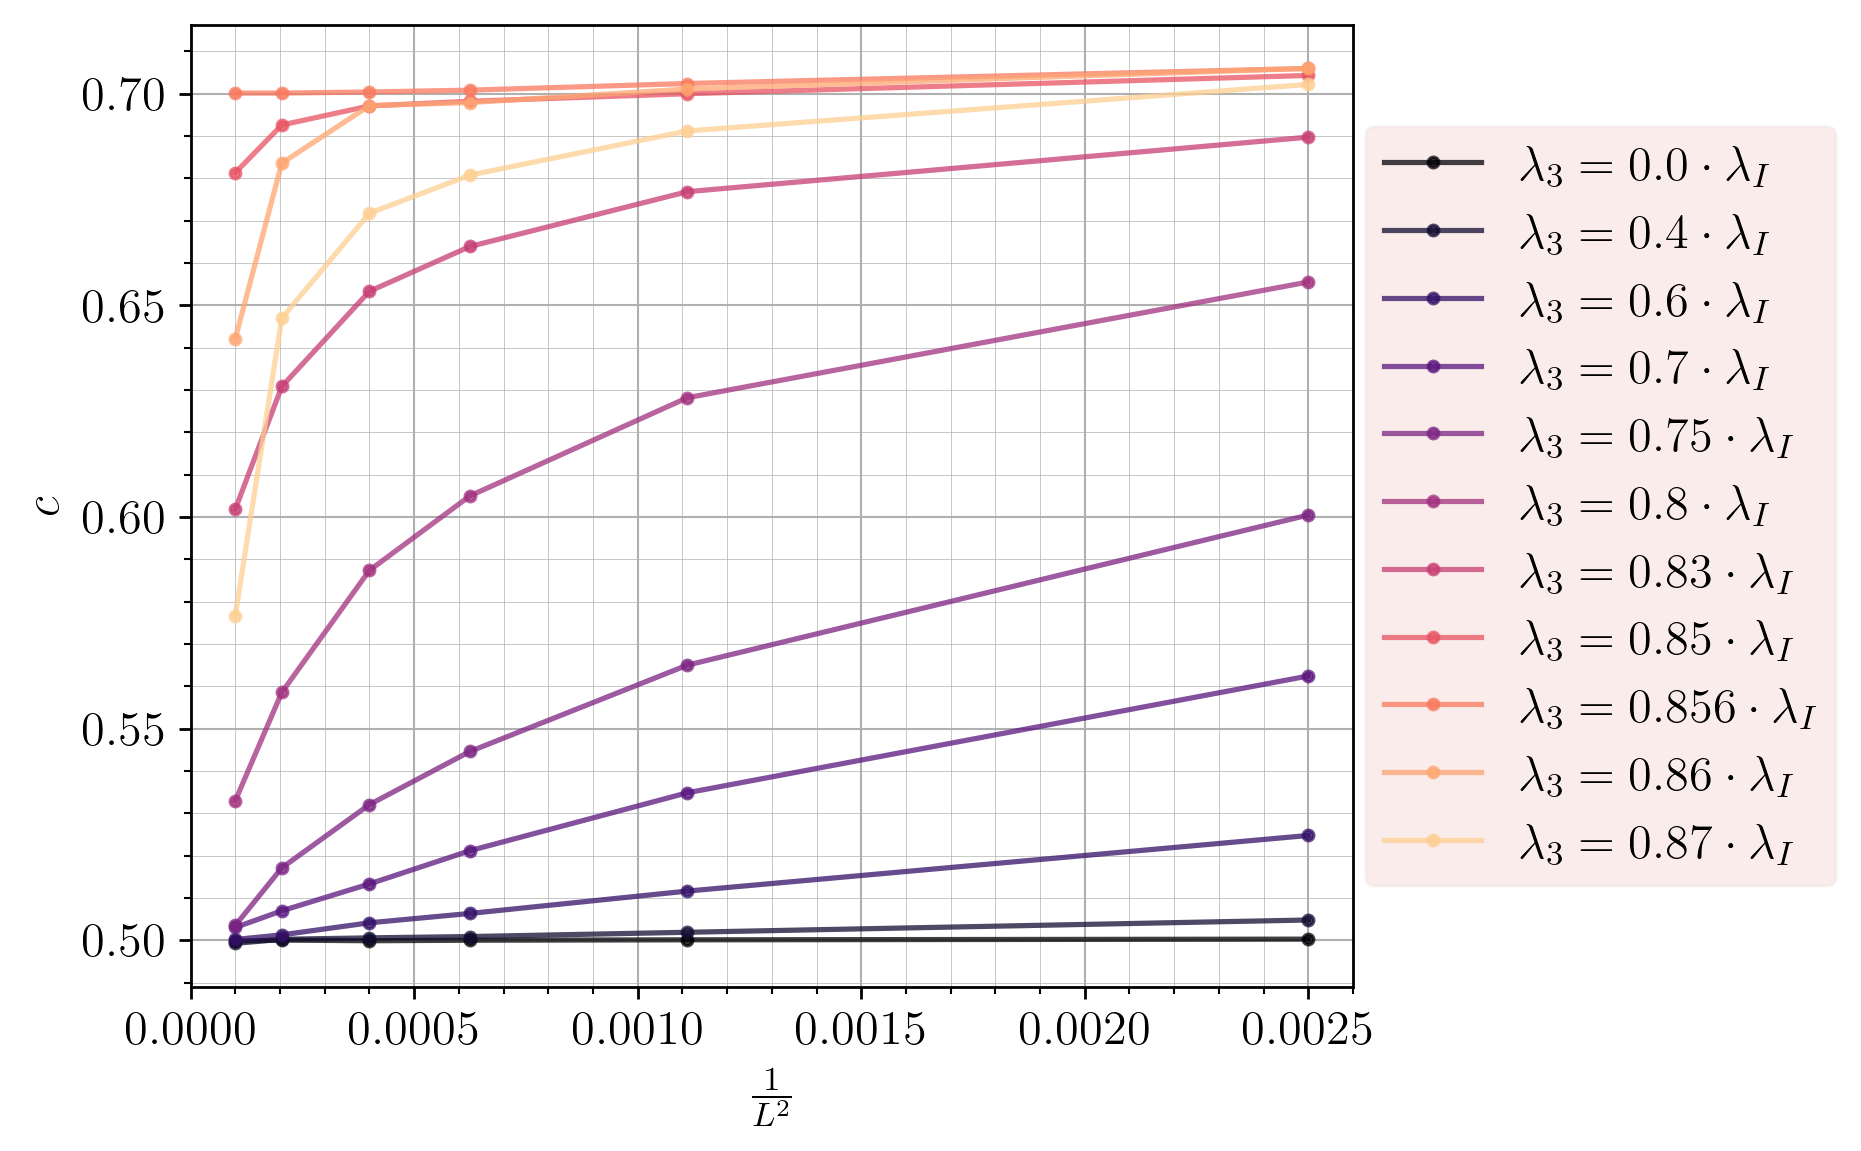
\includegraphics[scale=0.66]{../graphs/phase/pbc/J=1.0_h=1.0_i=1.0_c=0.0.png}
		\caption{Extrapolation of the central charge as $\lambda_3/\lambda_I$ is varied with PBCs for $\lambda_I=1$ and ground state variance $\sim 10^{-4}$.}
		\label{fig:phasePBCs}
	\end{figure}

	To have an insight of what happens at fixed length $L=30$ through the whole interval $\lambda_3/\lambda_I \in [0, 1]$, the central charge in computed for different values of this ratio on \autoref{fig:cWholeInterval}. It can be seen that $c$ is close to $0.5$ for $\lambda_3/\lambda_I<0.6$. Above this, $c$ tends to move aside this $0.5$ and increase towards $0.7$ which is reached for $\lambda_3/\lambda_I$ around $0.856$. After that point, $c$ decrease to reach $0$ approaching $\lambda_3/\lambda_I=1$ as the system there is expected to be gapped. This behavior is for a finite length $L=30$, and it is not excluded that the peak observed around $\lambda_3/\lambda_I=0.856$ narrows as $L$ in increased.

	\begin{figure}[h!]
		\centering
		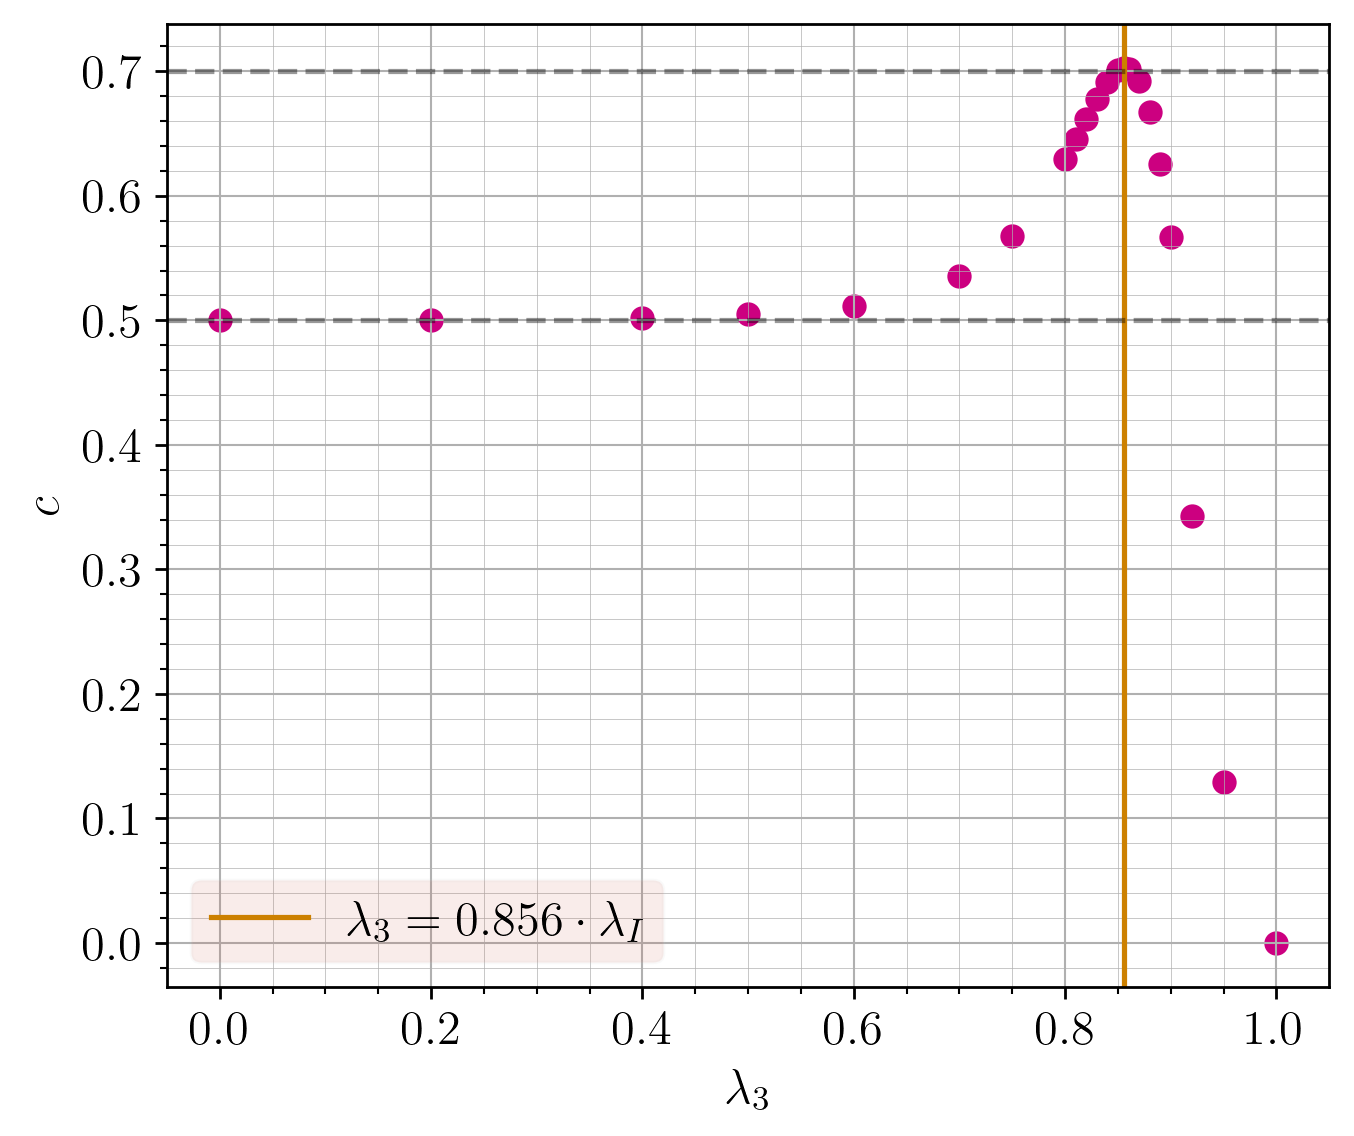
\includegraphics[scale=0.66]{../graphs/through/pbc/L=30.0_chi=100.0_J=1.0_h=1.0_i=1.0_c=0.0.png}
		\caption{Values of central charge as $\lambda_3/\lambda_I$ is varied at fixed length $L=30$, $\chi=100$ and PBCs. Dashed grey lines are added as guides for $c=1/2$ and $7/10$.}
		\label{fig:cWholeInterval}
	\end{figure}

	The use of PBCs was at first intended to compute universal ratios of energies at critical points described by CFT and around to further characterize them. This idea is that ratios of some energy differences are equal to ratios of conformal dimensions difference of the CFT operator realizing the state with the corresponding energy. This is somehow the same idea than building the conformal tower, except there is no need to use a lot of excitation energies and can use PBCs and ABCs. Hence, this will be entirely based on \cite{obrien2018, rahmani2015}. Three ratios will be computed numerically, have been listed in \cite{obrien2018} and are summarized in \autoref{tab:ratios}. The same notation will be used, namely $P^\pm_n$ and $A^\pm_n$ stand respectively for the $n^\text{th}$ excitation PBCs and ABCs energy in the $\pm$ sector of the Hamiltonian \eqref{eq:OF} corresponding to the eigenvalue of the parity operator $\mc F$.

	The results are presented on \autoref{fig:ratios} for different key values of $\lambda_3/\lambda_I$. The length goes from $10$ to $50$, due to the increase in computational cost from PBCs and from the application of the parity operator -- which tends to double the time needed for the same precision. The obtained ratios perfectly agree with those found in \cite{obrien2018} for the same range of lengths. For critical TFI, all values stay on the predicted line even for very small chains. The point $\lambda_3/\lambda_I=0.856$ is slightly off the predicted value for small lengths $10\to 30$ but the precision increases as $L$ increases. Just around it, $\lambda_3/\lambda_I=0.855, 0.857$, they seems to closely follow the behavior of $0.856$ still for small lengths. But starting from $L=30$, they move away from the TCI CFT and $0.855$ initiate its decrease towards Ising CFT, as does $0.8$ neatly, while $0.857$ start to follow a divergent curve as does $0.87$ as expected from $3$-fold degeneracy of the ground state in the gapped phase where $P^+_1 = P^+_0$. This will now be shown.

	\begin{table}[h!]
		\centering
		\renewcommand{\arraystretch}{1.3}
		\begin{tabular}{c|ccc}
			CFT & $R_1 = \frac{A^-_0 - P^+_0}{P^+_1 - P^+_0}$ & $R_2 = \frac{P^-_0 - P^+_0}{P^+_1 - P^+_0}$ & $R_3 = \frac{P^-_1 - P^+_0}{P^+_1 - P^+_0}$ \\
			\hline
			Ising & $\frac{1}{2}$ & $\frac{1}{8}$ & $\frac{9}{8}$ \\
			TCI & $\frac{7}{2}$ & $\frac{3}{8}$ & $\frac{35}{8}$
		\end{tabular}
		\caption{Values of the universal ratios of energy computed from corresponding CFT.}
		\label{tab:ratios}
	\end{table}

	\begin{figure}[h!]
		\centering
		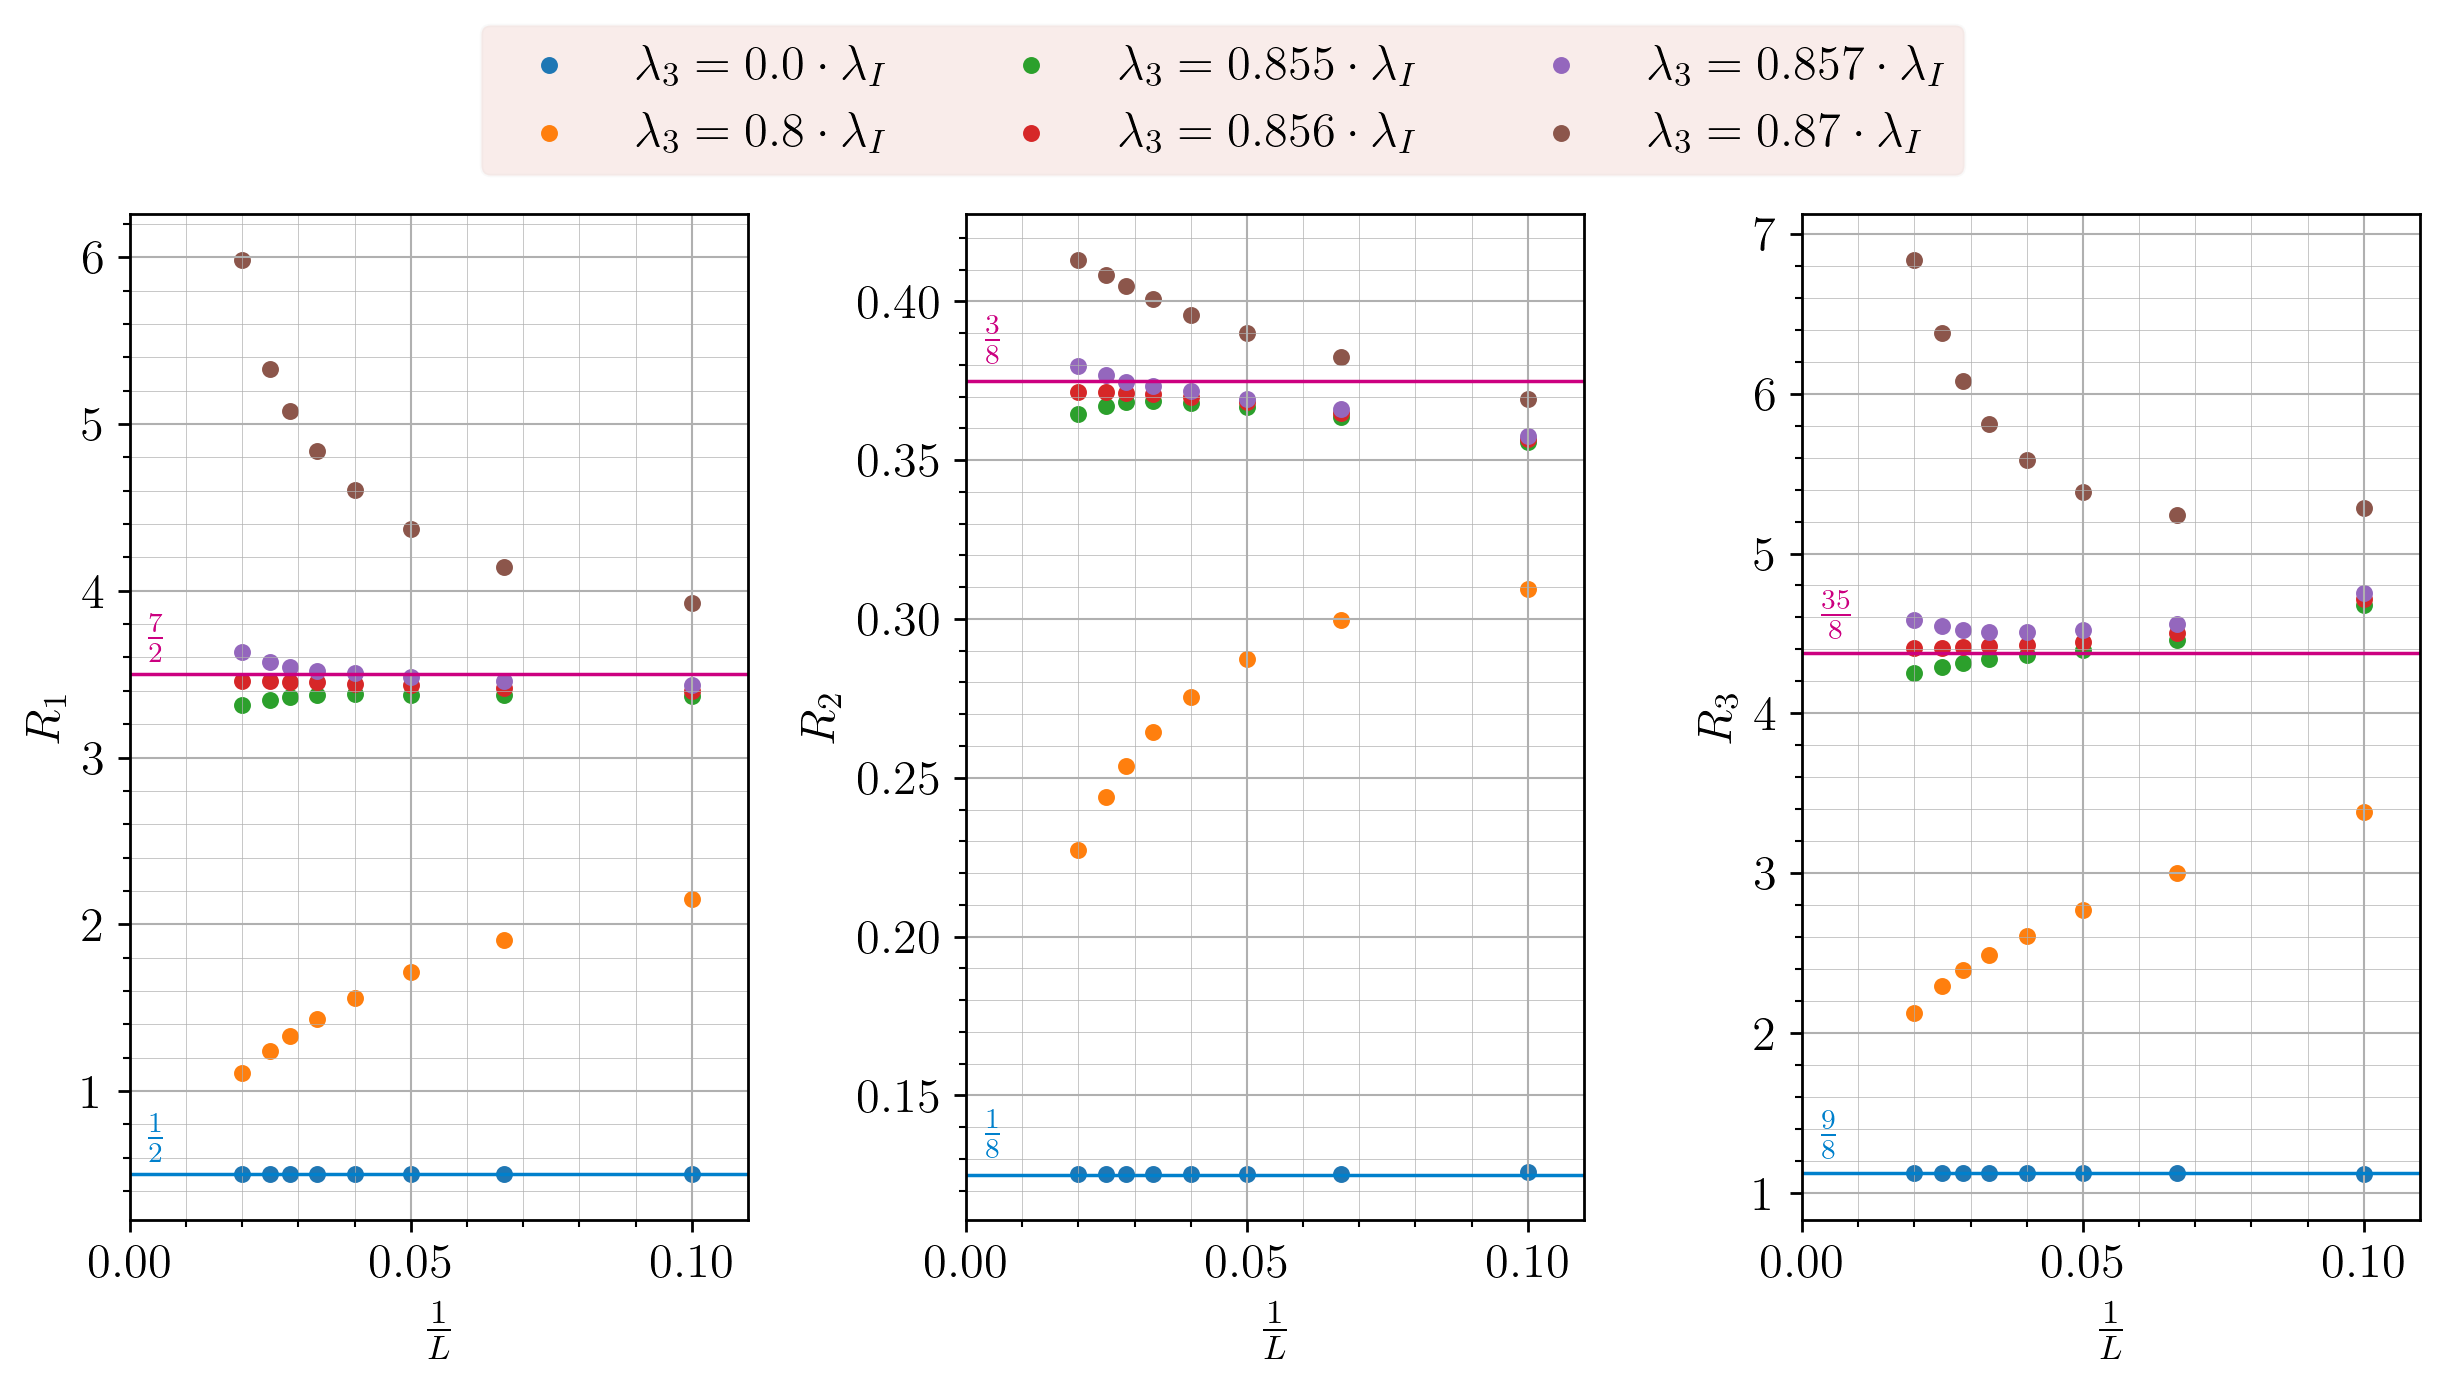
\includegraphics[scale=0.66]{../graphs/ratios/J=1.0_h=1.0_i=1.0_c=0.0.png}
		\caption{Extrapolation of the ratios \autoref{tab:ratios} for different key values of $\lambda_3/\lambda_I$ with ground state variance $\sim 10^{-4}$. CFT prediction are added with their corresponding values : cyan lines are for Ising CFT and magenta lines are for TCI CFT.}
		\label{fig:ratios}
	\end{figure}

	It has been shown that the ground state for $\lambda_3 = \lambda_I$, three ground states exist \cite{obrien2018}. It can be expected that the first three energies of the system from the ratios are $P^+_0$, $P^+_1$ and $P^-_0$ and since they have been shown to converge to the same value in the thermodynamic limit for $\lambda_3/\lambda_I > 0.856$, the differences between those energies are shown on \autoref{fig:degeneracy}. For $0\leq\lambda_3/\lambda_I \leq 0.856$ the system is critical, hence is gapless. Thus, any extrapolation of some energy difference must vanish as $L\to\infty$. Slightly above $0.856$, even though the system is gapped, finite size effects are expected to affect the energies so that they also tend to close the gap for large $L$. As $\lambda_3/\lambda_I$ is increased, only $2$ differences vanish for large lengths -- $P^-_0 - P^+_0$ and $P^+_1 - P^+_0$ --, whereas $P^-_1 - P^+_0$ stops at a finite value, indicating a gap. Since $P^-_1$ has been found to be the $4^\text{th}$ energy, this implies a $3$-fold degeneracy of the ground state for $\lambda_3/\lambda_I > 0.856$. It indeed has been checked that the ground states obtained for $\lambda_3=\lambda_I$ are $\ket{+\cdots +}$ and $\ket{-\cdots -}$ with the exact same energy $E_0 = -2\lambda_I L$. However, there is a third ground state that is not representable in MPS form, as described in \cite{obrien2018}.

	\begin{figure}[h!]
		\centering
		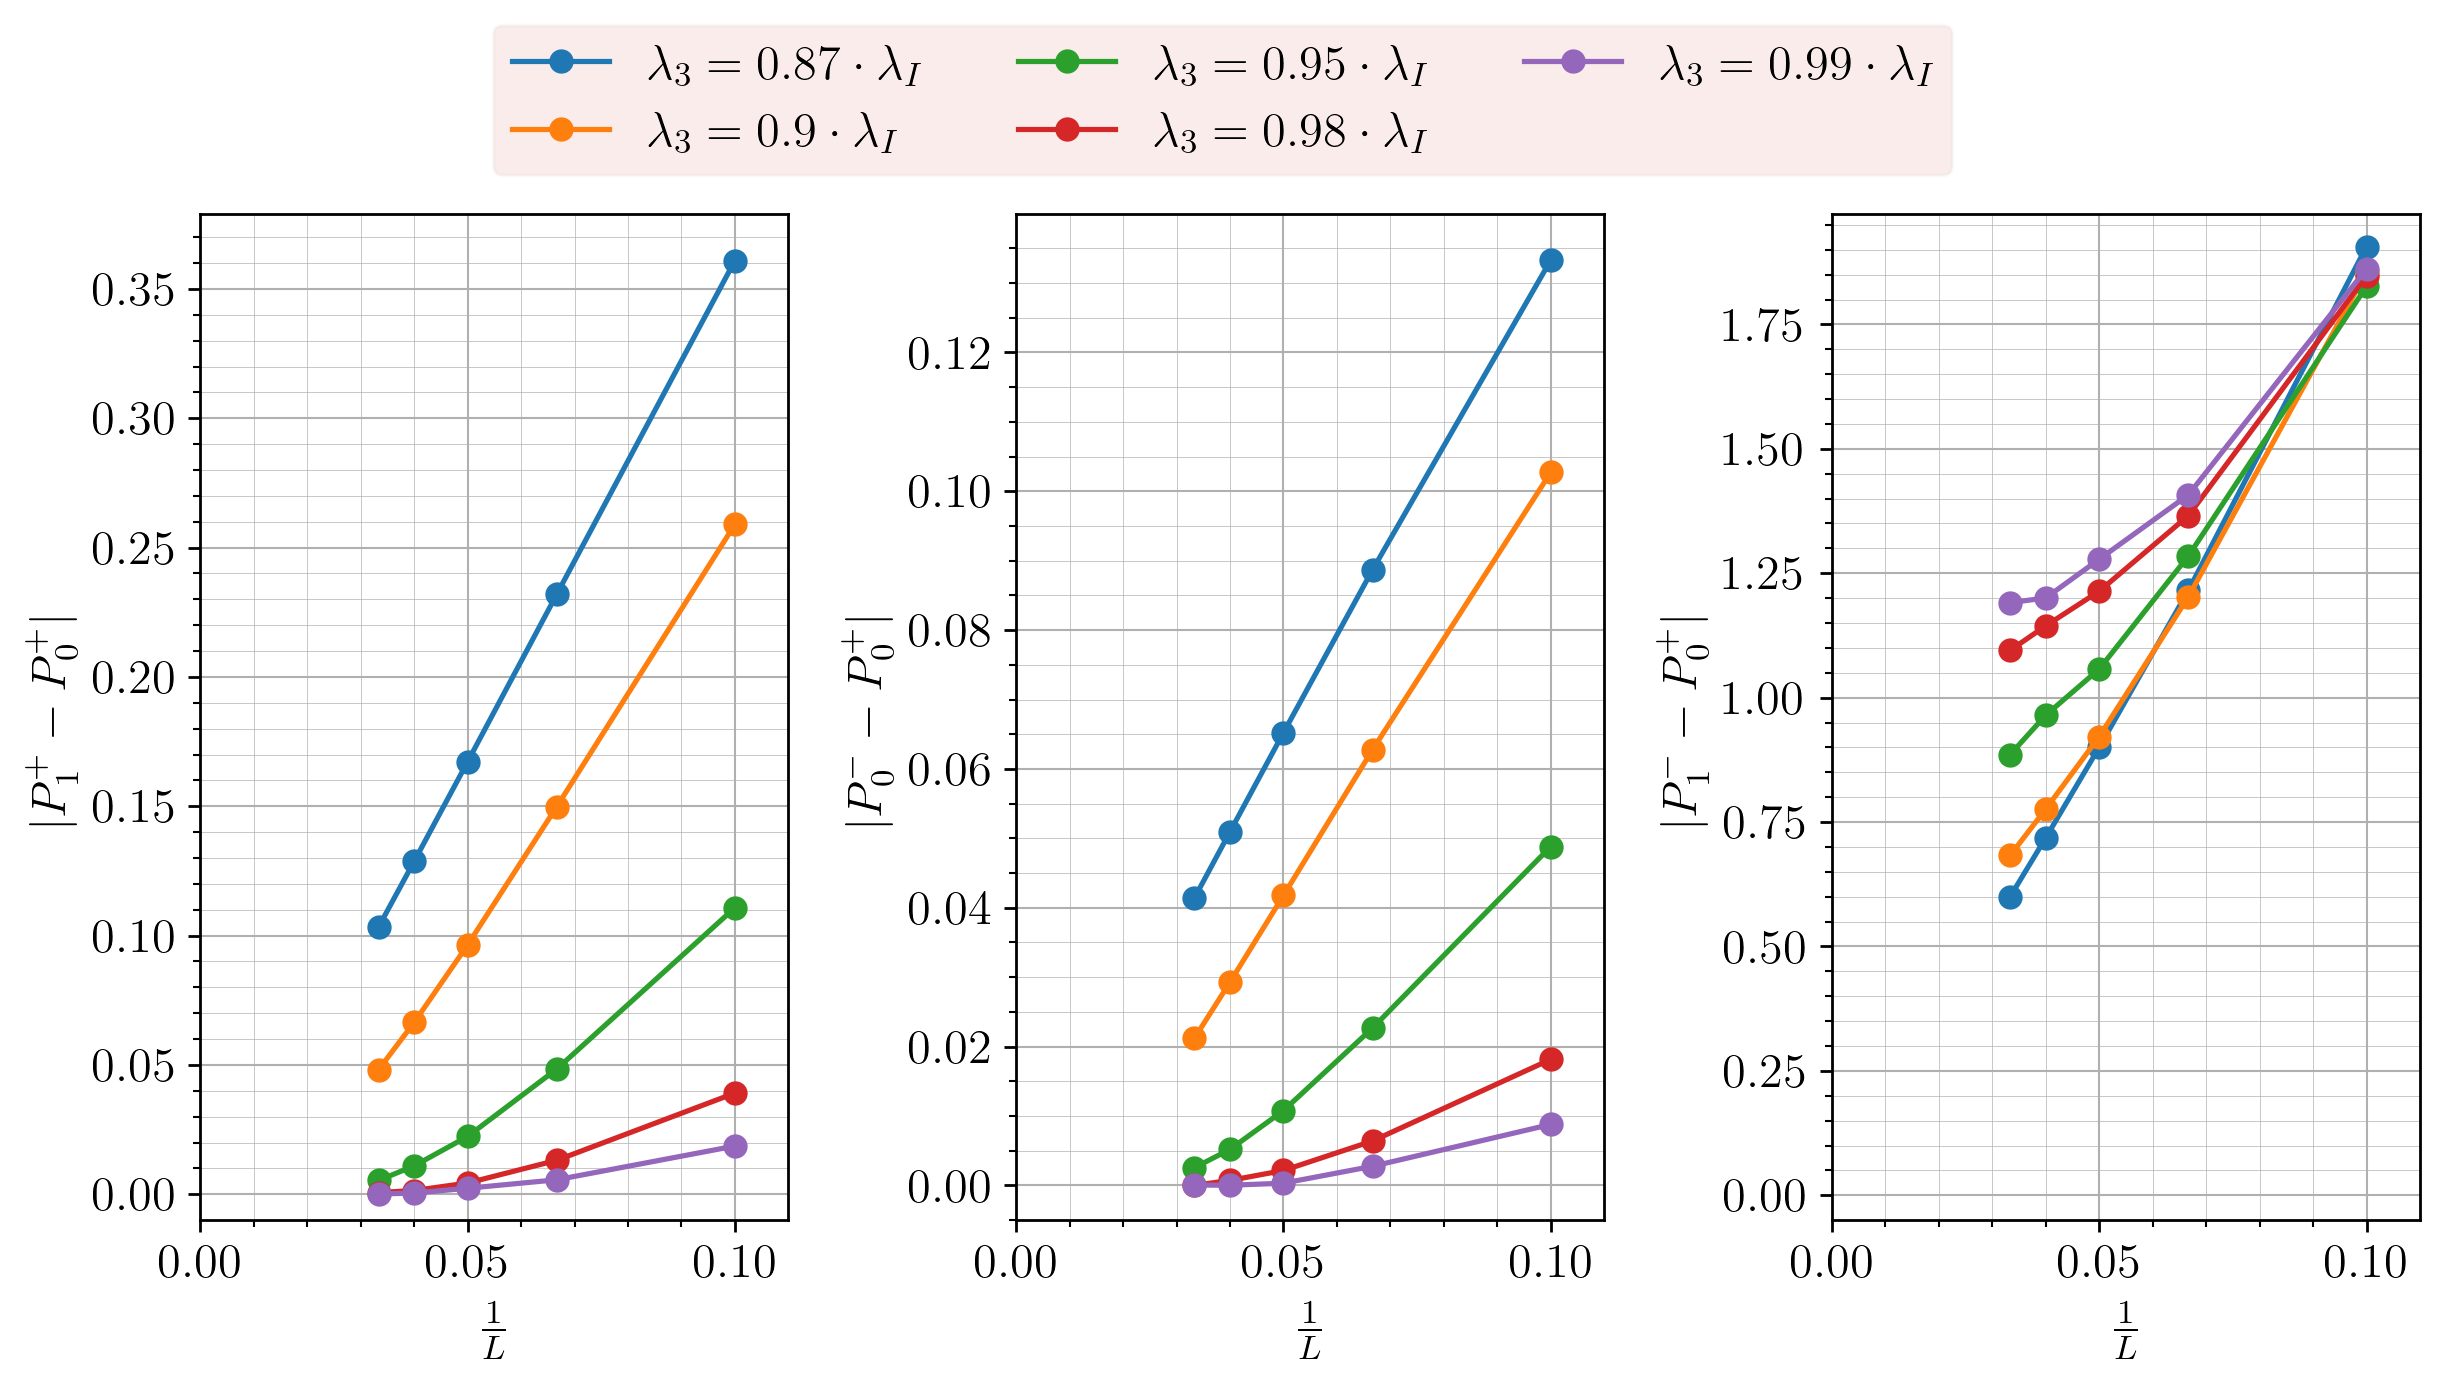
\includegraphics[scale=0.66]{../graphs/degeneracy/J=1.0_h=1.0_i=1.0_c=0.0.png}
		\caption{Extrapolation of the differences in energies for different values of $\lambda_3/\lambda_I$ with ground state variance $\sim 10^{-4}$. Each of them is chosen so that they compose the first low-lying excitation energies.}
		\label{fig:degeneracy}
	\end{figure}